\chapter{การเรียนรู้แบบลึก}
\label{chapter: ANN deep learning}
\index{deep learning}

\begin{verse}
``What you get by achieving your goals is not as important as what you become by achieving your goals.'' \\
Johann Wolfgang von Goethe
\end{verse}

โครงข่ายประสาทเทียม ความลึก $2$ ชั้น นั้น แม้จะสามารถทำงานหลายๆอย่างได้ดี ดังที่เห็นไปเช่น ตัวอย่างในบท~\ref{chapter: Applications of ANN}.
แต่ ความสามารถของ โครงข่ายประสาทเทียม ก็ยังห่างไกลจากเป้าหมายสูงสุด ของ ศาสตร์ปัญญาประดิษฐ์ ซึ่งคือ การสร้างเครื่องจักรที่มีความฉลาด เทียบเท่า ความฉลาดของมนุษย์.
มีความพยายามศึกษาหลายๆ แนวทาง เพื่อไปสู่เป้าหมายนั้น เช่น แนวทาง (Artificial General Intelligence)\cite{AGI2007a} , แนวทางที่พยายามจะรวม connectionism และ symbolism เข้าด้วยกัน\cite{Smolensky1988a, Smolensky1990a, ParkEtAl1995a}, แนวทางที่พยายามสร้างกรอบทำงานเชิงคำนวณรวมทั่วไป (generic computational framework)\cite{Prokopenko2014a}, แนวทางของ reinforcement learning, แนวทางของ hierarchical learning \cite{TaniNolfi1999a}, แนวทางการใช้บริบทประกอบ (context-aware learning)\cite{Turney1993a, SongEtAl2002a, FinkelEtAl2004a, SrinivasanEtAl2005a, GomesEtAl2011a} และ การเชื่องโยง มโนทัศน์ที่คล้ายคลึงกัน ในมุมมองต่างๆ, เป็นต้น รวมไปถึง การพยายาม จะนำ มิติที่เชื่อว่าจะช่วยเสริม ความสามารถ ของโครงข่ายประสาทเทียมไปในแนวทางนั้น เช่น active learning, transfer learning, เป็นต้น

ถึงแม้จะมีความพยายามดังกล่าวมานี้ สถานะปัจจุบัน ของศาสตร์และศิลป์ ของวิทยาการปัญญาประดิษฐ์ ก็ยังห่างไกล จากเป้าหมายสูงดังกล่าว.

\begin{verse}
``Only a small community has concentrated on general intelligence.
No one has tried to make a thinking machine . . .
The bottom line is that we really haven't progressed too far toward a truly intelligent machine. 
We have collections of dumb specialists in small domains; 
the true majesty of general intelligence still awaits our
attack. . . .
We have got to get back to the deepest questions of AI and general
intelligence...''
\\– Marvin Minsky
\\as interviewed in Hal’s Legacy, edited by David Stork, 2000.
\end{verse}

อย่างไรก็ดี ความก้าวหน้าล่าสุด ที่สร้างความตื่นเต้น กับ วงการปัญญาประดิษฐ์ และ คอมพิวเตอร์โดยรวม ไปจนถึง ผู้สนใจทั่วไป คือ แนวทางของการเรียนรู้แบบลึก (Deep Learning) ที่นอกจากจะทำงานในลักษณะการเรียนรู้แบบมีผู้สอนได้ดีแล้ว ยังเสมือนเป็นการรวมการการเรียนรู้แบบไม่มีผู้สอนเข้าไปได้ด้วย และ ยังเปิดทางให้กับ การทำ transfer learning, และ hierarchical representation ด้วย.
หากจะเริ่มต้น กล่าวถึง การเรียนรู้แบบลึก, แม้แนวคิดจะมีมานานมากพอๆกับ จุดกำเนิดของโครงข่ายประสาทเทียมเอง และ วิธีการแพร่กระจายย้อนกลับเองก็สามารถนำมาใช้ได้.
แต่การประยุกต์ใช้ โครงข่ายประสาทเทียมแบบลึก นั้นจำกัดอยู่มาก, จนกระทั่งการค้นพบที่สำคัญ ในปีี 2006 \cite{HintonSalakhutdinov2006a} ที่พบ วิธีการฝึกโครงข่ายประสาทเทียมแบบลึกได้อย่างมีประสิทธิภาพ.
หลักจากนั้น ก็มีการศึกษา การเรียนรู้แบบลึก อย่างกว้างขว้าง และ การเรียนรู้แบบลึก ก็กลายเป็น ศาสตร์และศิลป์ ที่สำคัญ สำหรับ ศาสตร์หลายๆแขนง \cite{Jones2014a, Schmidhuber2015a,MNIST20150311,DahlSainathHinton2013a,DengEtAl2013a, 
ErhanEtAl2010a,CaetanoDosSantoEtAl2015,RamsundarEtAl2015,
ChenEtAl2014a,MaEtAl2015a,XiongEtAl2015a} เช่น computer vision, speech recognition, natural language processing, drug discovery เป็นต้น.
การเรียนรู้แบบลึก มีความสำคัญ มีการใช้งานที่กว้างขวาง และศักยภาพสูงมาก จน
MIT Technology Review 2013 ได้ยกให้ การเรียนรู้แบบลึก (deep learning) เป็น 1 ใน 10 breakthroughs ของปี 2013.
ในขณะที่ รายการของปี 2014 ได้ยกให้ Neuromorphic Processing Unit เป็น 1 ใน breakthorughs ของปี.
Neuromorphic Processing Unit (NPU) \cite{MerollaEtAl2014a} ซึ่งคือ ฮาร์ดแวร์ที่โครงสร้างออกแบบเฉพาะ สำหรับ การใช้งานโครงข่ายประสาทเทียมหลากหลายรูปแบบ (รวมถึง โครงสร้างแบบลึก).
สถาปัตยกรรมนี้ ต่างจาก von Neumann machine ที่เป็นแนวคิดหลักของคอมพิวเตอร์ในปัจจุบัน อย่างสิ้นเชิง.
ผู้อ่านที่สนใจ เรื่อง NPU สามารถศึกษาได้ จาก งานที่สำคัญของ เมอโรลาและคณะ จาก IBM \cite{MerollaEtAl2014a}.

หัวข้อ~\ref{deep learning: self-taught learning} อภิปรายแนวคิดของ self-taught learning ซึ่งเป็นงานศึกษาถึงการใช้ การเรียนรู้แบบไม่มีผู้สอน มาช่วยเรียนลักษณะที่สำคัญของข้อมูล เพื่อ เพิ่มประสิทธิภาพในการเรียนรู้แบบมีผู้สอน.
เนื้อหา self-taught learning นำมาจาก บทความของรายนะและคณะ\cite{RainaEtAl2007a}.
โดยถึงแม้ งานของรายนะและคณะ จะเป็นโมเดลเชิงเส้น ที่มีลักษณะตื้น แต่ หลักการที่ นำข้อมูลไม่มีฉลาก มาปรับโมเดล ยกหนึ่งก่อน เพื่อที่จะหา representations ที่ดีของข้อมูล,
ซึ่งภายหลัง representations ที่ดี จะช่วยให้ การปรับโมเดลอย่างละเอียด ด้วย ข้อมูลที่มีฉลาก จะทำได้มีประสิทธิภาพ มากขึ้น.
แนวคิดนี้ เป็นหลักการเดียวกันกับ แนวทาง ที่นำมาใช้กับการฝึกโครงสร้างแบบลึก ด้วยการทำ pre-train ที่จะกล่าวต่อไปในหัวข้อ~\ref{deep learning: deep learning}.

\section{การเรียนรู้แบบสอนตนเอง}
\label{deep learning: self-taught learning}
\index{self-taught learning}

เนื้อหาในหัวข้อนี้ มาจากงานของ รายนะและคณะ \cite{RainaEtAl2007a} ที่ศึกษา การนำ ข้อมูลที่ไม่มีฉลาก มาช่วยเพิ่มประสิทธิภาพ การเรียนรู้แบบมีผู้สอน. 
%ที่ต้องการข้อมูลพร้อมฉลาก 
และ เสนอแนวทาง ที่เรียกว่า ``self-taught learning'' หรือ ``การเรียนรู้แบบสอนตนเอง''.

\paragraph{Conventional supervised learning:} สถานการณ์ที่ทำๆกันมา ของ การทำโมเดล สำหรับ งานการเรียนรู้แบบมีผู้สอน คือ เราจะมี ข้อมูลตัวอย่าง พร้อมกับ เฉลย ที่มักเรียก ``ฉลาก'':
งานหาค่าถดถอย, ฉลาก ก็คือ ค่าเอาต์พุต ที่ต้องการ;
งานจำแนกกลุ่ม, ฉลาก ก็คือ กลุ่มที่ถูกต้อง.

\paragraph{Issue:} ดังนั้น หากจะทำ การทำโมเดล สำหรับ งานการเรียนรู้แบบมีผู้สอน, เราต้องมี ตัวอย่างที่ดี และ เพียงพอ: มี ข้อมูลตัวอย่าง พร้อม ฉลาก และ ตัวอย่างก็ควรจะมีจำนวน และ ความหลากหลายเพียงพอ ที่จะช่วยให้ โมเดลได้เรียนรู้ ความน่าจะเป็น ของ ความสัมพันธ์ ระหว่างข้อมูลและฉลาก, การกระจายของข้อมูล, และ การกระจายของฉลาก.
แต่ สำหรับ งานหลายๆประเภท เช่น การรู้จำวัตถุ (object recognition), การรู้จำเสียง (speech recognition), การจำแนกชนิดบทความ (text article classification), การแปลภาษา (machine translation), เป็นต้น, สถานการณ์ คือ มันเป็นงานที่ซับซ้อน และต้องการข้อมูลตัวอย่างจำนวนมาก;
แต่ ข้อมูลที่มีฉลาก (ที่ถูกต้อง และ เกี่ยวข้อง) มีจำนวนน้อย เกินไป ที่จะใช้ทำโมเดลที่ดีได้.
อย่างไรก็ตาม โอกาสก็คือ มี ข้อมูลที่ไม่มีฉลาก เป็นจำนวนมาก (มี รูปภาพ, ไฟล์เสียง, บทความ ข้อเขียน ข้อความ ต่างๆ อยู่มากมาย หลากหลายภาษา ในอินเตอร์เนต).
งานการเรียนรู้แบบมีผู้สอน แบบดั้งเดิม ไม่ได้ใช้ประโยชน์ จาก ข้อมูลที่ไม่มีฉลากที่มีอยู่เป็นจำนวนมาก เหล่านี้ เลย.

\paragraph{Proposed solution:} แนวคิด ของ self-taught learning คือ การใช้ ข้อมูลที่ไม่มีฉลาก เช่น รูปภาพ (หรือ ไฟล์เสียง หรือ เอกสารข้อความ) มาช่วยในการปรับโมเดลก่อน.
นำข้อมูลไม่มีฉลากจำนวนมาก จะปรับให้โมเดลสรุปได้ลักษณะที่สำคัญ ของข้อมูลมาก่อน
แล้วค่อย นำข้อมูลที่มีฉลาก มาปรับแต่งโมเดลในขั้นตอนสุดท้าย เพื่อให้ได้งานที่ต้องการ.

โดย รายนะและคณะ ได้แจกแจงความแตกต่างระหว่าง self-taught learning กับ งานการเรียนรู้ของเครื่องแบบอื่นๆ เช่น supervised learning (งานเรียนรู้แบบมีผู้สอน), semi-supervised learning (งานเรียนรู้แบบกึ่งมีผู้สอน), transfer learning (งานโยกย้ายการเรียนรู้) พร้อมภาพประกอบ ที่แสดงในรูป~\ref{fig: deep self-taught compares}.
หากต้องการสร้างโมเดล เพื่อ แยกภาพของ ช้าง กับ แรด,
supervised learning ต้องการ ภาพตัวอย่าง ของทั้งช้าง และ แรด พร้อม ฉลาก ระบุว่า เป็นภาพ ช้าง หรือ แรด จำนวนมาก;
semi-supervised learning\footnote{
เช่น เราใช้ ภาพของช้างกับแรดที่มีฉลาก มาฝึกโมเดล และ ทายฉลาก ของภาพที่ไม่มีฉลาก;
แล้ว ใช้ ภาพที่ไม่มีฉลาก มาประกอบกับ ฉลากที่ทาย มาฝึกโมเดลต่อ.
ทำเช่นนี้ จะเสมือนว่า เราได้มีข้อมูลที่มีฉลากเยอะขึ้น.
ดู [cite Tom Mitchell's semisupervised learning] เพิ่มเติมสำหรับ Semi-supervised learning.} 
ต้องการ ภาพตัวอย่าง ของทั้งช้าง และ แรด ที่มี ฉลาก และ สามารถเสริมด้วย ภาพช้าง และ ภาพแรด ที่ไม่มีฉลากได้;
transfer learning\footnote{
ดู [cite Quan Yan's Transfer Learning] เพิ่มเติมสำหรับ Transfer learning.
}
ต้องการ ข้อมูลตัวอย่างของงานที่ต้องการ พร้อมฉลาก และ สามารถเสริมได้ด้วย ตัวอย่างของงานที่คล้ายคลึงกัน
เช่น สมมติว่า งานจำแนกม้าและแพะ สามารถนำมาช่วย งานจำแนกช้างและแรดได้,
transfer learning ก็สามารถใช้ ภาพแพะ และ ภาพม้า พร้อมฉลาก มาเสริมได้;
รายนะ และ คณะ ชี้แจงว่า self-taught learning เหมาะสมกับ สภาพทั่วๆไปมากกว่า คือ สำหรับ งานจำแนกช้างและแรด, seft-taught learning สามารถใช้ ภาพอะไรก็ได้มาเสริมการทำงาน โดย 
ไม่จำเป็นว่า ภาพที่มาเสริมจะต้องเป็น ภาพช้าง หรือ ภาพแรด (เงื่อนไขของ semi-supervised learning)
หรือ
ไม่จำเป็นว่า ภาพที่มาเสริมจะต้องมีฉลากประกอบ (เงื่อนไขของ transfer learning).

%
\begin{figure}
\begin{center}
\includegraphics[width=5.5in]{04ANNDeep/MLCompare.png}
\end{center}
\caption{ภาพจาก Raina et al 2007 เปรียบเทียบ supervised learning, semi-supervised learning, transfer learning, และ self-taught learning.}
\label{fig: deep self-taught compares}
\end{figure}
%

\paragraph{Self-taught learning formulation:}
ให้ ข้อมูลตัวอย่างพร้อมฉลาก $N$ ตัวอย่าง: $\{ x_l^{(1)}, y^{(1)} \}$, $\{ x_l^{(2)}, y^{(2)} \}$, $\ldots \{ x_l^{(N)}, y^{(N)} \}$ (i..i.d. จาก distribution $\mathcal{Q}$)
โดย $x_l^{(i)} \in \Re^D$ เป็นอินพุตเวกเตอร์ (โดย subscript $l$ ระบุว่า มีฉลาก; อินพุตแต่ละตัวมี $D$ มิติ)
และ $y^{(i)} \in \{ 1, 2, \ldots, C \}$ เป็น ฉลากของ $x_l^{(i)}$.
และ ให้ ข้อมูลตัวอย่างที่ไม่มีฉลาก $K$ ตัวอย่าง: 
$x_u^{(1)}$, $x_u^{(2)}$, $\ldots$, $x_u^{(K)} \in \Re^D$
โดย $x_u^{(j)}$ ไม่จำเป็นต้องมาจาก distribution เดียวกับ $x_l^{(i)}$ หรือ แม้แต่ ไม่จำเป็นต้องเกี่ยวข้องกับฉลากเดียวกัน.
เช่น ดังแสดงในรูป~\ref{fig: deep self-taught compares}, $x_l^{(i)}$ อาจเป็นภาพของช้าง หรือ ภาพของแรด;
ส่วน $x_u^{(j)}$ อาจเป็นภาพแม่น้ำ ภาพภูเขา ซึ่งไม่ได้มาจาก distribution เดียวกับ ภาพช้าง หรือ ภาพแรด และ ก็ไม่ได้เกี่ยวข้องกับฉลาก ``ช้าง'' หรือ ``แรด'' เลย.

สังเกตุ $x_l$ และ $x_u$ มี มิติเท่ากัน.
หากสามารถแก้ข้อจำกัดนี้ของการเรียนรู้ของเครื่องได้ (รวมถึง ความสามารถในการจัดการ กับ บางส่วนของอินพุต), ศักยภาพของการเรียนรู้ของเครื่อง คงจะเพิ่มขึ้น อย่างก้าวกระโดด.

ด้วย ข้อมูลที่มีฉลาก และ ข้อมูลที่ไม่มีฉลาก, จุดประสงค์ ของ self-taught learning คือ การหา hypothesis $h: \Re^D \rightarrow \{1, \ldots, C\}$,
 หรือ พูดง่ายๆคือ หาโมเดล $h$ ที่ใช้ ทำนายกลุ่ม ของอินพุต, 
 โดย พยายามเลียนแบบ ความสัมพันธ์ ระหว่าง อินพุตของข้อมูลที่มีฉลาก และ ฉลากของมัน.
โมเดล $h$ นี้ จะถูกทดสอบด้วย ข้อมูลที่มาจาก distribution $\mathcal{Q}$ (แบบเดียวกับ ตัวอย่างข้อมูลที่มีฉลาก).

อัลกอริทึ่มของ self-taught learning แบ่งเป็น $3$ ขั้นตอน.
ขั้นตอนแรก คือ การหาลักษณะสำคัญพื้นฐานของข้อมูล, หรือ เบซิส (bases) , โดย การใช้ ข้อมูลที่ไม่มีฉลาก $\{ x_u^{(1)}, \ldots, x_u^{(K)} \}$ ที่มีอยู่เป็นจำนวนมาก
มาแก้ปัญหา~\ref{eq: deep self-taught unsupervised stage}.

\begin{eqnarray}
  \min_{b,a} & \sum_i \| x_u^{(i)} - \sum_j a_j^{(i)} b_j \|_2^2 + \beta \| a^{(i)} \|_1
\label{eq: deep self-taught unsupervised stage} \\
  \mbox{s.t.} & \| b_j \|_2 \leq 1, \forall j \in 1, \ldots, M
\nonumber  
\end{eqnarray} 
เมื่อ $M$ แทนจำนวนลักษณะสำคัญพื้นฐาน ซึ่ง ลักษณะสำคัญพื้นฐาน แทนด้วย เบซิสเวกเตอร์ (basis vectors), $b = \{ b_1, b_2, \ldots, b_M \}$ ที่แต่ละเวกเตอร์ $b_j \in \Re^D$.
ทบทวนว่า $D$ คือ จำนวนมิติของอินพุต.
และ $a = \{ a^{(1)}, a^{(2)}, \ldots, a^{(K)} \}$ ที่แต่ละ $a^{(i)} \in \Re^M$ ทำหน้าที่เป็นเวกเตอร์ค่าน้ำหนักของข้อมูล $i$.
เวกเตอร์ $a^{(1)}$ ทำหน้าที่เหมือนเป็น ตัวกระตุ้น (activation) หรือ ตัวควบคุมว่าจะเลือกใช้เบซิสไหนบ้าง มากน้อยเท่าไร เพื่อมาผสมกัน ให้ได้ค่าประมาณใกล้เคียงกับ ข้อมูล $x_u^{(i)}$.

แนวคิดคือ ข้อมูล $x_u^{(i)}$ ที่มี $D$ มิติ จะสามารถถูกประมาณได้ด้วย โมเดล ผลรวมเชิงเส้นของลักษณะสำคัญ $\sum_{j=1}^M a_j^{(i)} b_j$.
สมการ~\ref{eq: deep self-taught unsupervised stage} หาค่า ลักษณะสำคัญ $b$ ที่ทำให้ โมเดล $\sum_{j=1}^M a_j^{(i)} b_j$ ประมาณค่า $x_u^{(i)}$ ได้ใกล้เคียงที่สุด.

เทอมหลัง ในสมการ~\ref{eq: deep self-taught unsupervised stage} เป็น  regularization term  เพื่อบังคับ ไม่ให้ค่าน้ำหนัก $a^{(i)}$ ใหญ่เกินไป,
โดย $\beta$ ทำหน้าที่ เป็น regularization parameter\footnote{
ค่า $\beta$ เป็นพารามิเตอร์ของอัลกอริทึ่ม ที่ต้องเลือกให้เหมาะสม.
ดูหัวข้อ~\ref{sec: regularization} สำหรับพื้นฐานเรื่องเรกูลาไรเซชั่น หรือ \cite{ChongZak2ndEd} สำหรับมุมมองทั่วไปของวิธีการหาค่าดีที่สุด ที่ $\beta$ จะเรียกว่า Lagrange multiplier}
การคุมไม่ให้ค่า $a^{(i)} = |a^{(i)}_1| + |a^{(i)}_2| + \ldots + |a^{(i)}_M|$ ไม่มาก เพื่อ ให้บังคับให้ค่า $a^{(i)}_1, a^{(i)}_2, \ldots, a^{(i)}_M$ มีลักษณะหร็อมแหร็ม (sparse): มี $a^{(i)}_m$ ที่มีค่าไม่กี่ตัว ส่วนใหญ่มีค่าเป็น $0$ ซึ่งเทียบเท่ากับ มีไม่กี่เบซิสที่ถูกเลือกออกมา (เลือกเฉพาะลักษณะเด่นๆออกมา แล้วตัดรายละเอียดที่ไม่สำคัญทิ้งไป)\footnote{
จุดประสงค์ คือ เราต้องการคุมให้ $a^{(i)}$ แต่ละตัวมีลักษณะหร็อมแหร็ม โดยผ่านกลไกของ เทอม $\|a^{(i)}\|$.
แต่ ด้วยกลไกที่เราใช้ ก็มีความเป็นไปได้ว่า แทนที่เราจะได้ $a^{(i)}$ ที่มีลักษณะหร็อมแหร็ม,
เราอาจได้ $|a^{(i)}_1|, \ldots, |a^{(i)}_M|$ ที่มีค่าน้อยๆทุกตัว ก็ได้ เช่น
$\| [0.2, 0.2, 0.2, 0.2, 0.2]^T \| = 1.0 = \| [0.9, 0.1, 0, 0, 0]^T \|$, แต่จริงแล้วเราต้องการแบบหลัง (หร็อมแหร็ม) มากกว่า เพราะ แบบบอกชัดเจนว่า ลักษณะสำคัญพื้นฐาน คือ เบซิสที่หนึ่ง และ มีลักษณะของเบซิสที่สองปนนิดหน่อย.
}.


หลังจากได้ลักษณะสำคัญพื้นฐาน $b$ แล้ว 
%ค่าน้ำหนักของลักษณะสำคัญต่างๆ จะช่วยบอกว่า ลักษณะเด่นของข้อมูลนั้น 
%เช่น
%หาก ลักษณะสำคัญในภาพ ได้แก่ $b_1$ ลักษณะมีวัตถุแหลมค่อนข้างยาว, $b_2$ ลักษณะวัตถุแหลมค่อนข้างยาวมีสีอ่อน, $b_3$ ลักษณะวัตถุแหลมค่อนข้างยาวมีอันเดียว, เป็นต้น และ หากภาพที่หนึ่งเราได้ค่าน้ำหนักที่แทน
%
ขั้นตอนที่สอง เป็น ขั้นตอนแปลงข้อมูลที่เราสนใจ ให้เป็น ค่าน้ำหนักของลักษณะสำคัญ หรือ เรียกสั้นๆว่า ลักษณะสำคัญ (features): $x_l^{(i)} \mapsto a_l^{(i)}$.
%เช่น หากภาพที่เราต้องการจำแนก มีขนาด $112 \times 92$ พิกเซล,
%แต่ละภาพจะมีขนาด $10,304$ มิติ;
%และ เราเลือกทำลักษณะสำคัญ $200$ ลักษณะ ($M = 200$), 
เ%ราจะแปลง ภาพที่หนึ่ง $x^{(1)} \in \Re^{10,304}$ ไปเป็น น้ำหนักของลักษณะสำคัญ $a^{(1)} \in \Re^{200}$.
%หากทำเช่นนี้ เท่ากับเป็นการช่วยลดมิติของข้อมูล (dimension reduction)\index{dimension reduction} ทำให้ เราสามารถประมวลผลต่อไป ได้อย่างมีประสิทธิภาพมากขึ้น.
%หากเราทำลักษณะสำคัญได้ดี มิติที่ลดทอนหายไป จะไม่มีผลมาก.

%ขั้นตอนที่สอง ของ self-taught learning, 
เราหาค่า ลักษณะสำคัญ $a_l^{(i)}$ ได้โดย นำข้อมูลฝึกที่มีฉลาก $x_l^{(i)}$ มาแปลงเป็น ค่าน้ำหนักของลักษณะสำคัญ $a_l^{(i)}$, โดยการแก้สมการ~\ref{eq: deep self-taught mapping stage},
\begin{eqnarray}
  a_l^{(i)} = \arg \min_{a^{(i)}} \| x_l^{(i)} - \sum_{j=1}^M a_j^{(i)} b_j \|_2^2 + \beta \| a^{(1)} \|_1.
\label{eq: deep self-taught mapping stage}  
\end{eqnarray}

เทอม $\sum_{j=1}^M a_j^{(i)} b_j$ เป็นการประมาณ $x_l^{(i)}$ ด้วย sparse linear combination ของเบซิสเวกเตอร์ $b$.
ค่าน้ำหนักของลักษณะสำคัญ $a_l^{(i)}$ เป็น เสมือน representation ใหม่ ของ อินพุต $x_l^{(i)}$.

ซึ่ง representation $a_l^{(i)}$ นี้ จะใช้ร่วมกับ ฉลาก $y^{(i)}$ เพื่อใช้ฝึกโมเดลจำแนกประเภท ซึ่งเป็นขั้นตอนสุดท้าย ของอัลกอริทึ่ม self-taught learning.
ตาราง~\ref{tbl: deep self-taught learning} สรุป อัลกอริทึ่ม self-taught learning.
หมายเหตุ SVM ย่อจาก Support Vector Machine เป็น วิธีทางการเรียนรู้ของ
เครื่องที่นิยมอีกวิธี สำหรับงานจำแนกกลุ่ม (ดู \cite{Burges1998A, CortesVapnik1995a, SchoelkopfEtAl1999a, ChangEtAl2011a} เพิ่มเติมสำหรับ SVM)

%
\begin{table}[hbtp]
\caption{Raina et al 2007's Self-taught Learning with Sparse Coding}
\begin{center}
\begin{tabular}{|l|}
\hline
$\mathbf{input}$ \\
\quad Labeled training set $T = \{ (x_l^{(1)}, y^{(1)}), (x_l^{(2)}, y^{(2)}), \ldots, (x_l^{(N)}, y^{(N)})\}$. \\
\quad Unlabeled data $\{ x_u^{(1)}, x_u^{(2)}, \ldots, x_u^{(K)} \}$. \\
$\mathbf{output}$ Learned classifier $\mathcal{C}$ for the classification task. \\
$\mathbf{algorithm}$ \\

\quad (1) Using unlabeled data $\{ x_u^{(i)} \}$, obtain bases $b$ by solving\\
\quad \quad \quad $ \min_{b,a} \sum_i \| x_u^{(i)} - \sum_j a_j^{(i)} b_j \|_2^2 + \beta \| a^{(i)} \|_1$ \\
\quad \quad \quad s.t. $\| b_j \|_2  \leq 1$, $\forall j \in 1, \ldots, M_1$. \\

\quad (2) Compute representations for the classification task: \\
\quad \quad \quad $ a_l^{(i)} = \arg \min_{a^{(i)}} \| x_l^{(i)} - \sum_j a_j^{(i)} b_j \|_2^2 + \beta \| a^{(i)} \|_1$. \\

\quad (3) Using new training set $\hat{T} = \{ (a_l^{(1)}, y^{(1)}), (a_l^{(2)}, y^{(2)}), \ldots, (a_l^{(N)}, y^{(N)})\}$, \\
train a classifier $\mathcal{C}$ (, e.g., ANN, SVM). \\

\hline
\end{tabular} 
\end{center}
\label{tbl: deep self-taught learning}
\end{table}

สังเกตุ ทั้ง สมการ~\ref{eq: deep self-taught unsupervised stage} และ ~\ref{eq: deep self-taught mapping stage} มีการใช้ $L_2$ และ $L_1$ regularization (เทอมหน้า และ เทอมหลังตามลำดับ).
สมการ~\ref{eq: deep L1} และ~\ref{eq: deep L2} แสดง $L_1$ และ $L_2$ regularization ตามลำดับ,

\begin{eqnarray}
 \| \mathbf{v} \|_1 &=& \sum_i |v_i|
\label{eq: deep L1} \\
 \| \mathbf{v} \|_2 &=& \sqrt{ \sum_i (v_i)^2 }
\label{eq: deep L2}.
\end{eqnarray}

รายนะและคณะ ได้แสดงความเห็นว่า การใช้ เทอม $L_1$ จะสามารถคุมให้ได้ ลักษณะสำคัญ $a_l^{(i)}$ ที่หร็อมแหร็มได้ดีกว่า.
ตัวอย่างเช่น สมมติ เวกเตอร์ $a_l^{(i)}$ มีค่า $[0.2, 0.2, 0.2, 0.2, 0.2]^T$, 
ผล regularization จาก $L1$: 
\begin{eqnarray}
\| a_l^{(i)} \| &=& |0.2| + |0.2| + |0.2| + |0.2| + |0.2|
\nonumber \\
  &=& 1
\nonumber .
\end{eqnarray}
ในขณะที่ ผล regularization จาก $L2$:
\begin{eqnarray}
\| a_l^{(i)} \|_2 &=& \sqrt{0.2^2 + 0.2^2 + 0.2^2 + 0.2^2 + 0.2^2}
\nonumber \\
  &=& 0.447
\nonumber .
\end{eqnarray}

ค่า $[0.2, 0.2, 0.2, 0.2, 0.2]^T$ ไม่หร็อมแหร็ม.
เราไม่ชอบ ให้การกระตุ้น $a_l^{(i)}$ เป็นแบบนี้,
ดังนั้น ด้วยกลไกของ เรกูลาไรเซชั่น ที่มีฤทธิ์ลงโทษ (ไปเพิ่มค่าฟังชั่นจุดประสงค์, นิพจน์~\ref{eq: deep self-taught unsupervised stage}),
ผลของเรกูลาไรเซชั่น สำหรับ ค่าที่เราไม่ชอบ, เช่น $[0.2, 0.2, 0.2, 0.2, 0.2]^T$, ควรมีค่ามาก.
จะเห็นว่า เทอม $L1$ จะให้ผลลงโทษที่รุนแรงกว่า เทอม $L2$,
เมื่อค่าของ $\| a_l^{(i)} \|$ ไม่ได้หร็อมแหร็ม.

พูดอีกอย่างหนึ่ง คือ การใช้ค่าสัมบูรณ์ทำให้ ผลลงโทษของเทอมเรกูลาไรเซชั่น มีค่าตาม ขนาดค่ากระตุ้น, 
เช่น ค่าการกระตุ้น $(a_l^{(i)})_m$ เป็น $0.2$, ผลลงโทษของเทอมเรกูลาไรเซชั่น ก็สะท้อนออกมา $0.2$.

รูป~\ref{fig: deep L1 L2 Norm} แสดงเปรียบเทียบ ค่า $x^2$ กับ $|x|$ ในช่วง $x \in [-1,1]$.
จากรูป จะเห็นว่า $L_1$ regularization ซึ่งใช้ค่าสัมบูรณ์กับแต่ละค่าของเวกเตอร์ $a_l^{(i)}$ จะให้ผล regularization ที่แรงกว่า การใช้ค่ากำลังสอง:
ที่ค่าการกระตุ้นเดียวกัน เช่น $0.2$, ค่าสัมบูรณ์ก็จะเป็น $0.2$ ซึ่ง คือ ผลลงโทษมีค่า ตามค่ากระตุ้นที่ใช้.
ในขณะที่ ค่ากำลังสองจะเป็น $0.04$, ซึ่งแม้ จะมีผลลงโทษ แต่ ผลลงโทษ มีค่าอ่อนกว่า ค่ากระตุ้นที่ใช้\footnote{
การใช้ $L2$ regularization, จะมีการถอดรากที่สองในขั้นตอนสุดท้าย ทำให้ ผลลงโทษสุดท้าย ไม่ได้ขึ้นกับ ค่ากำลังสองของค่ากระตุ้นค่าใดค่าเดียว.
อย่างไรก็ตาม การอภิปรายในที่นี้ชี้ให้เห็นคร่าวๆว่า เทอมกำลังสอง ไม่ได้มีประสิทธิภาพ เท่ากับ เทอมค่าสัมบูรณ์ ในการบังคับ การหร็อมแหร็ม (sparsity).
%อย่างไรก็ตาม ผลโดยรวมดังแสดงในตัวอย่างก่อนหน้า เช่น $$a_l^{(i)} = [0.2, 0.2, 0.2, 0.2, 0.2]^T$
%แสดงให้เห็นว่า $L2$ regularization (ผ่านกลไก ของ ค่ากำลังสอง ของแต่ละค่ากระตุ้น) ไม่ได้ส่งเสริม ให้การกระตุ้น $a_l^{(i)}$ มีค่าหร็อมแหร็ม ได้เท่ากับ $L1$ regularization.
}.
พูดง่ายๆ คือ การใช้ค่าสัมบูรณ์ในกลไกของเรกูลาไรเซชั่น ส่งเสริมการหร็อมแหร็มได้ดีกว่า.
%
ดู \cite{Ng2004a} สำหรับ การอภิปรายเรื่อง $L_2$ และ $L_1$ regularization รวมถึง ประโยชน์ของการใช้ $L_1$ regularization ในการคุมค่าพารามิเตอร์ ของโมเดล.

%
\begin{figure}
\begin{center}
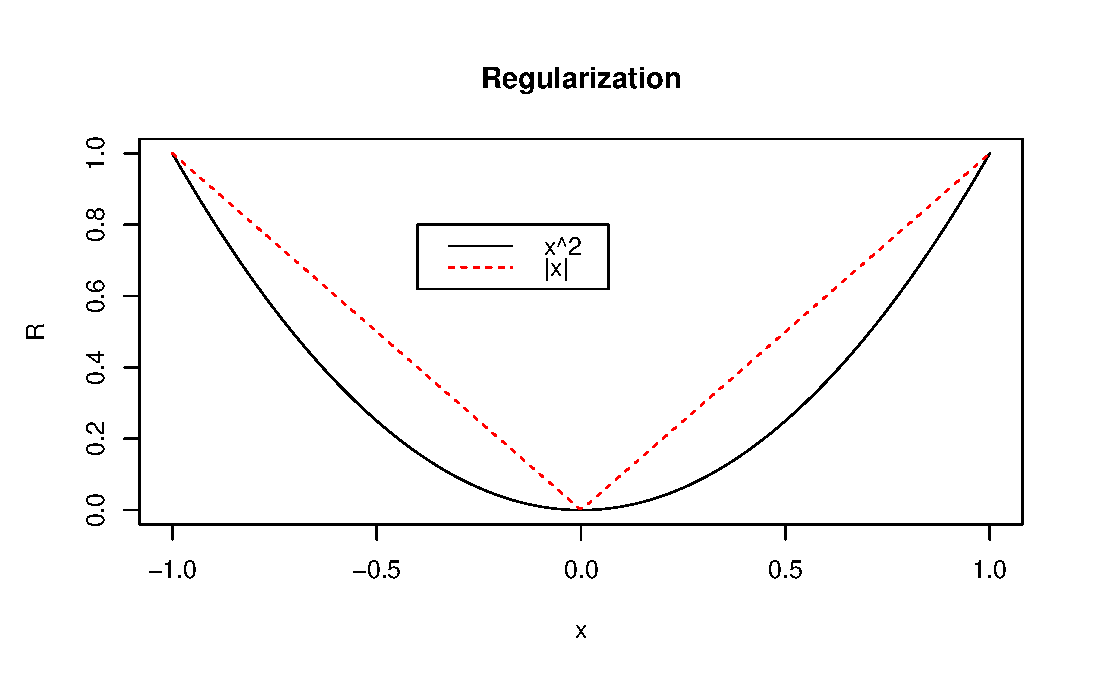
\includegraphics[width=6in]{04SelfTaught/L1L2Norm.eps}
\end{center}
\caption{เปรียบเทียบค่า $x^2$ กับ $|x|$ ในช่วง $x \in [-1,1]$}
\label{fig: deep L1 L2 Norm}
\end{figure}
%

\paragraph{ตัวอย่าง}
รายนะและคณะได้แสดงตัวอย่างของเบซิส ดังแสดงในรูป~\ref{fig: deep Raina et al Fig 2}.
ภาพซ้าย แสดง ตัวอย่างของเบซิส ที่เรียนจาก image patches (ขนาด $14 \times 14$ pixels) ที่สุ่มออกมาจากภาพทิวทัศน์ต่างๆ.
นั่นคือ ให้ $x_u^{(i)}$ เป็นเวกเตอร์ ค่าของพิกเซล $14 \times 14 = 196$ ค่า.
สังเกตุว่าลักษณะของเบซิสที่ได้ คล้ายกับ เป็น ตัวตรวจจับขอบต่างๆที่ผสมเป็นภาพ (edge detection).
ในภาพแสดง เบซิส 32 ตัว: $b_1, b_2, \ldots, b_{32}$ โดยที่ เบซิสแต่ละตัวเป็นเวกเตอร์ขนาด $196$.
ภาพขวา แสดง ตัวอย่างของเบซิส 4 ตัว ที่เรียนจาก sound samples (ขนาด 25 ms) ที่สุ่มมาจากสัญญาณเสียง.
ลักษณะของเบซิสที่ได้ คล้ายกับ เป็น ตัวตรวจจับความถี่ต่างๆที่ผสมเป็นเสียง.
เราจะได้เบซิสเหล่านี้ออกมาหลังจากขั้นตอนที่หนึ่ง (แก้ปัญหา~\ref{eq: deep self-taught unsupervised stage})

%
\begin{figure}
\begin{center}
\begin{tabular}{cc}
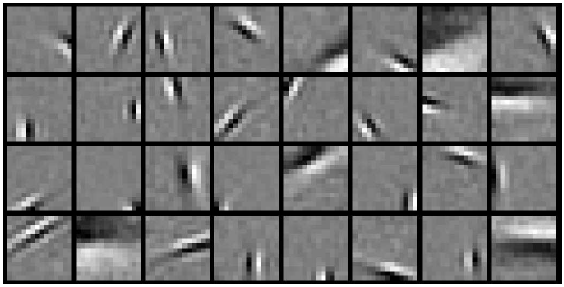
\includegraphics[width=2.5in]{04SelfTaught/RainaEtAlFig2a.png} 
& 
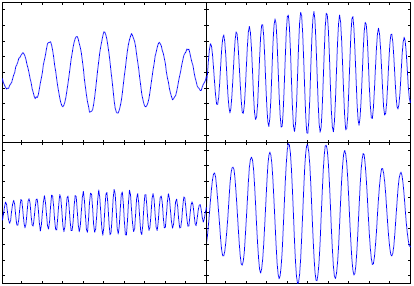
\includegraphics[width=2.5in]{04SelfTaught/RainaEtAlFig2b.png}
\end{tabular} 
\end{center}
\caption{ภาพจาก Raina et al 2007 แสดงตัวอย่าง ของ เบซิส (bases):
ภาพซ้าย เป็น ตัวอย่างของเบซิส 32 ตัว ที่เรียนจาก image patches (ขนาด $14 \times 14$ pixels) ที่สุ่มออกมาจากภาพทิวทัศน์ต่างๆ;
ภาพขวา เป็น ตัวอย่างของเบซิส 4 ตัว ที่เรียนจาก sound samples (ขนาด 25 ms) ที่สุ่มมาจากสัญญาณเสียง}
\label{fig: deep Raina et al Fig 2}
\end{figure}
%

หลังจากขั้นตอนที่สอง เราจะได้ ลักษณะสำคัญ $a^{(i)}$'s ซึ่งคือ การกระตุ้นของลักษณะพื้นฐาน (สมการ~\ref{eq: deep self-taught mapping stage}).
แต่ละค่ากระตุ้น ในเวกเตอร์ลักษณะสำคัญ $a^{(i)} = [a^{(i)}_1, a^{(i)}_2, \ldots, a^{(i)}_M]^T$ จะบอกค่าน้ำหนักของ เบซิส ที่จะมาประกอบ กลับไปเพื่อ แทน อินพุต $x_l^{(i)}$.
รูป~\ref{fig: deep Raina et al Fig 3} แสดง เบซิส 3 ตัว กับ ค่ากระตุ้นของแต่ละตัว เพื่อประกอบกลับเป็น อินพุต $x_l^{(i)}$ (โดยประมาณ):
$a_{142}^{(i)} = 0.6$, $a_{381}^{(i)} = 0.8$, $a_{497}^{(i)} = 0.4$ หรือ 
\begin{eqnarray}
a^{(i)} = 
[0, \ldots 0, 0.6, 0, \ldots, 0, 0.8, 0, \ldots, 0, 0.4, 0, \ldots, 0]^T
\nonumber .
\end{eqnarray}
สังเกตุ การกระตุ้น $a^{(i)}$ (ซึ่งคือ ``ลักษณะสำคัญของอินพุตตัวที่ $i$'') มีค่าหร็อมแหร็ม: มีค่ามากๆอยู่ไม่กี่ค่า ค่าการกระตุ้นส่วนใหญ่เป็น $0$.
นี่คือ การที่ การกระตุ้น $a^{(i)}$ สามารถเลือกลักษณะพื้นฐานที่สำคัญของอินพุต $i$ ออกมาได้.
ในลักษณะเดียวกับ ที่เราจำใบหน้าคนจากลักษณะพื้นฐานที่สำคัญ เช่น ตา หู จมูก ปาก โดยละรายละเอียดปลีกย่อยอื่นๆทิ้งไป.
%
ดังนั้น เราอาจมอง การกระตุ้น $a^{(i)}$ นี้ได้ว่า เป็นเสมือนกับ การแทนอินพุต $i$ ในระดับที่สูงขึ้น (higher level representation) หรือ การสรุปย่อ (abstract) ของอินพุต $i$.
และ เราก็จะสามารถใช้ $a^{(i)}$ ไปเป็นอินพุต ของอัลกอริทึ่มเพื่อจำแนกกลุ่ม เช่น SVM หรือ โครงข่ายประสาทเทียม ได้ต่อไป.

%
\begin{figure}
\begin{center}
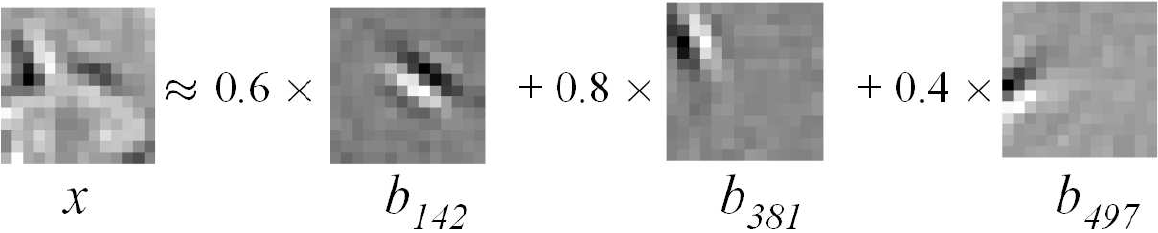
\includegraphics[width=5in]{04SelfTaught/RainaEtAlFig3.png}
\end{center}
\caption{ภาพจาก รายนะและคณะ 2007; 
อินพุตแต่ละตัว สามารถถูกประมาณได้ด้วย ผลรวมของลักษณะพื้นฐานตามค่าน้ำหนัก;
ลักษณะพื้นฐาน (เบซิส) จะใช้ร่วมกันสำหรับ อินพุตทุกตัว;
แต่ค่าน้ำหนักที่ต่างกันของเบซิสต่างๆ จะผสม ค่าประมาณออกมาให้คล้ายกับอินพุตแต่ละตัว;
อินพุต $x^{(i)}$ แต่ละตัว  จะมี ชุดของค่าน้ำหนักเฉพาะ ของตัวเอง;
ชุดของค่าน้ำหนัก สำหรับ อินพุต $x^{(i)}$ คือ การกระตุ้น $a^{(i)}$.}
\label{fig: deep Raina et al Fig 3}
\end{figure}
%

\begin{minipage}{5.5in}
{\small
\begin{shaded}
สังเกตุว่า แทนที่จะ แปลงรูปขนาดใหญ่ เป็น เบซิส และ ค่าน้ำหนัก โดยตรง, 
รายนะและคณะ สุ่มรูปย่อย (image patches) ที่แต่ละรูปที่ขนาดเท่ากัน และ หาค่า เบซิส และ ค่าน้ำหนัก จาก รูปย่อยเหล่านี้แทน.
วิธีนี้เป็นวิธีที่นิยมมาก ในงาน computer vision เพราะ จะช่วยให้ เราสามารถ จำแนก วัตถุเดียวกัน ที่อยู่ตำแหน่งต่างกันในภาพได้.

หลังจากได้ เบซิส แล้ว, ค่าน้ำหนัก ที่จะใช้ อธิบายภาพใหญ่ จะได้จากทำเทคนิค sliding window,
ที่เราจะหยิบ ส่วนของภาพใหญ่ ที่มีขนาดเท่ากับ image patch ออกมา และ หาค่าน้ำหนักของเบซิสต่างๆที่ ส่วนนั้น จากนั้นก็ขยับไปหยิบส่วนข้างๆ ทำไปจนครบทั้งภาพ\footnote{
การขยับไปส่วนข้างๆ อาจขยับไปทีละพิกเซล หรือ ขยับด้วยก้าวที่หยาบกว่าก็ได้ ขึ้นกับ ประเภทของงาน และ ทรัพยากรที่สนับสนุน.
การขยับไปทีละพิกเซล อาจจะให้ผลที่ดีที่สุด ละเอียดที่สุด แต่ก็จะทำให้ได้ ค่าน้ำหนักเป็นจำนวนมาก ซึ่ง ก็จะเปลืองทรัพยากรการคำนวณ ทั้งเวลา และ หน่วยความจำ.
}.
และ ค่าน้ำหนักของเบซิสต่างๆ ที่ส่วนต่างๆของภาพ จะเป็นลักษณะที่ใช้บรรยายภาพนั้น และใช้เป็นอินพุต สำหรับ อัลกอริทึ่มเพื่อจำแนกกลุ่ม ต่อไป.

รายนะและคณะ กล่าวถึง การใช้ขั้นตอนพิเศษ เพื่อช่วยจัดการทรัพยากรการคำนวณได้มีประสิทธิภาพมากขึ้น, สำหรับรายละเอียด แนะนำให้ศึกษาโดยตรงจาก \cite{RainaEtAl2007a}.

รูป~\ref{fig: deep Raina et al Fig 4} แสดงค่าน้ำหนักของเบซิสต่างๆ ($4$ เบซิส) ที่ส่วนต่างๆของภาพใหญ่: แต่ละค่าพิกเซลในรูปขวามือ คือ ค่าน้ำหนักของเบซิสนั้นที่ส่วนนั้นของภาพ.
พิกเซลสีขาว แทน ค่าน้ำหนักที่เป็นบวกมากๆ และ พิกเซลสีดำ แทน ค่าน้ำหนักที่เป็นลบมากๆ.
จะเห็นว่า ค่าน้ำหนักที่ได้ จะเสมือนเป็น ตัวตรวจจับ ลักษณะของส่วนของภาพที่ใกล้กับเบซิสนั้นๆ.

\end{shaded}
}

\end{minipage}

%
\begin{figure}
\begin{center}
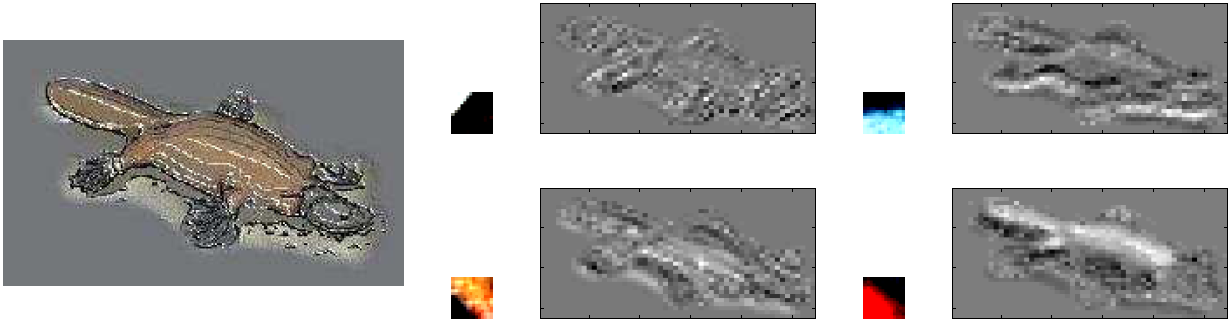
\includegraphics[width=5in]{04SelfTaught/RainaEtAlFig4.png}
\end{center}
\caption{ภาพจาก รายนะและคณะ 2007 (ควรดูเป็นภาพสี); ซ้ายมือ เป็น ภาพใหญ่ต้นฉบับ ของ ตุ่นปากเป็ด; ขวามือ เป็น ค่าน้ำหนักของเบซิสต่างๆที่ได้จากตำแหน่งต่างๆของภาพตุ่นปากเป็ด โดยมีภาพขยายของเบซิสแสดงอยู่ทางซ้าย (ไอคอนเล็กๆ); ค่าน้ำหนักที่ได้เรียงตามตำแหน่งที่ได้จากภาพต้นฉบับ โดย สีพิกเซลขาว แทนค่าน้ำหนักที่เป็นบวกมาก และ สีดำแสดงค่าเป็นลบมาก; สังเกตุว่าค่านำ้หนักที่ได้ ทำตัวเสมือนเป็น การตรวจจับลักษณะของภาพที่ตำแหน่งนั้นๆที่ใกล้เคียงกับเบซิส}
\label{fig: deep Raina et al Fig 4}
\end{figure}
%


ตาราง~\ref{tbl: deep Raina et al 2007 results} นำตัวอย่างผลประเมินของวิธีการเรียนรู้แบบสอนตนเอง จากงานของ รายนะและคณะ 2007\cite{RainaEtAl2007a} มาแสดง.
รายนะและคณะใช้ PCA (Principle Component Analysis) ซึ่งเป็น วิธีดั้งเดิมและยังเป็นที่นิยม ใช้สำหรับการ แปลงอินพุต ไปสู่ ลักษณะสำคัญ มาเพื่อเปรียบเทียบ.
ในตาราง, Unlabeled SC หมายถึง การใช้การเรียนรู้แบบสอนตนเอง และ ใช้ข้อมูลที่ไม่มีฉลาก มาประกอบ; Labeled PCA หมายถึง การใช้ PCA กับเฉพาะอินพุตของข้อมูลที่มีฉลาก;
และ Labeled SC หมายถึง การใช้การเรียนรู้แบบสอนตนเอง แต่ใช้เพียง ข้อมูลที่มีฉลากเท่านั้น.
ในตารางนำผลการประเมินจากงาน 4 อย่าง: (1) Handwritten character recognition ที่จำแนก ค่าความเข้มของพิกเซลทั้ง $28 \times 28$ พิกเซล เป็นตัวอักษร `a' ถึง `z' โดยใช้ ภาพลายมือเขียนของตัวอักษร `a' ถึง `z' เป็น ข้อมูลฝึกที่มีฉลาก และ ใช้ ภาพของลายมือเขียนตัวเลข `0' ถึง `9' เป็นข้อมูลที่ไม่มีฉลาก;
(2) Font character recognition ที่จำแนก ค่าความเข้มของพิกเซลทั้ง $28 \times 28$ พิกเซล เป็นตัวอักษร `a'/`A' ถึง `z'/`Z'
โดยใช้ ภาพฟอนต์ของ ตัวอักษร `a'/`A' ถึง `z'/`Z' เป็นข้อมูลฝึกที่มีฉลาก และ ใช้
ภาพของลายมือเขียนตัวอักษร `a' ถึง `z' เป็นข้อมูลที่ไม่มีฉลาก;
(3) Webpage classication จำแนก bag-of-words\footnote{วิธี bag-of-words เป็น รูปแบบ การแทน ข้อความ ด้วยค่าความถี่ของคำที่พบในบทความ ซึ่งเป็นวิธีหนึ่งที่นิยมใช้ศาสตร์การประมวลผลภาษาธรรมชาติ (natural language processing)} ของหน้าเวป ไปเป็น ประเภทของเวป
โดยใช้ หน้าเวปที่มีการจำแนกประเภทแล้ว เป็น ข้อมูลฝึกที่มีฉลาก
และใช้ บทความข่าว จาก Reuters newswire เป็นข้อมูลที่ไม่มีฉลาก;
และ (4) UseNet article classification จำแนก bag-of-words ของ UseNet posts ไปเป็น ประเภทของโพสต์
โดยใช้ UseNet Posts ที่มีการจำแนกประเภทแล้ว เป็น ข้อมูลฝึกที่มีฉลาก
และใช้ บทความข่าว จาก Reuters newswire เป็นข้อมูลที่ไม่มีฉลาก.

จากผลที่นำเสนอ จะเห็นว่า เมื่อจำนวนข้อมูลที่ใช้ฝึก อัลกอริทึ่มเพื่อจำแนกกลุ่ม มีจำนวนน้อยๆ, Unlabeled SC (การใช้การเรียนรู้แบบสอนตนเอง ประกอบการใช้ข้อมูลที่ไม่มีฉลาก) ช่วยให้ได้ผลการจำแนกที่ดีกว่า การใช้ PCA หรือ การเรียนรู้แบบสอนตนเองแต่ใช้เฉพาะข้อมูลที่มีฉลาก.
แต่เมื่อปริมาณข้อมูลมีมากขึ้น เช่น กรณี งานจำแนก รายมือเขียนตัวอักษร (Handwritten characters) กับข้อมูลฝึก 5000 ตัวอย่าง, 
ผลประโยชน์จากการใช้ ข้อมูลไม่มีฉลาก อาจเห็นไม่ชัดนัก.
ซึ่งเรื่องนี้ ก็สมเหตุสมผลดีที่ว่า หากเรามีข้อมูลสำหรับการฝึกมากพอ เราก็ไม่จำเป็นต้องใช้ ข้อมูลที่ไม่มีฉลากมาช่วย.
งานอื่นๆ ที่แสดงในตาราง อาจไม่ได้มีจำนวนข้อมูลฝึกมากพอจะทำเห็นแนวโน้มในแบบเดียวกัน.
%
สุดท้ายแล้ว การประเมินได้แสดงให้เห็นว่า การเรียนรู้แบบสอนตนเอง สามารถ ใช้ประโยชน์จาก ข้อมูลที่ไม่มีฉลาก เพื่อ เสริม ประสิทธิภาพ การทำงาน ของ การเรียนรู้แบบมีผู้สอนได้ โดยเฉพาะเมื่อ ปริมาณข้อมูลสำหรับฝึกมีน้อย.

%
\begin{table}[hbtp]
\caption{Accuracy on the self-taught learning tasks (ตารางที่ 7 ใน Raina et al 2007)}
\begin{center}
\begin{tabular}{|c|c|c|c|c|}
\hline
Domain & Training & Unlabled & \multicolumn{2}{c|}{Labeld} \\
\cline{4-5}
       & set size & SC       & PCA  & SC \\
\hline
              & 100  & 39.7\% & 36.2\% & 31.4\% \\
Handwritten   & 500  & 58.5\% & 50.4\% & 50.8\% \\
characters    & 1000 & 65.3\% & 62.5\% & 61.3\% \\
              & 5000 & 73.1\% & 73.5\% & 73.0\% \\
\hline
Font          & 100  & 7.0\%  & 5.2\%  & 5.1\% \\
characters    & 500  & 16.6\% & 11.7\% & 14.7\% \\
              & 1000 & 23.2\% & 19.0\% & 22.3\% \\
\hline
              & 4    & 64.3\% & 55.9\% & 53.6\% \\
Webpages      & 10   & 75.9\% & 57.0\% & 54.8\% \\
              & 20   & 80.4\% & 62.9\% & 60.5\% \\
\hline
UseNet 	      & 4    & 63.8\% & 60.5\% & 50.9\% \\
              & 10   & 68.7\% & 67.9\% & 60.8\% \\
\hline
\end{tabular} 
\end{center}
\label{tbl: deep Raina et al 2007 results}
\end{table}

%%%%%%%%%%%%%%%%%%%%%%%%%%%%%%%%%%%%%%%%%%%%%
\begin{minipage}{5.5in}
{\small
\begin{shaded}
การหาค่าดีที่สุด ในปัญหาที่มีข้อกำจัด (Constraint Optimization)
\index{constraint optimization}
\index{soft constraint}
\index{hard constraint}
\\
นิพจน์~\ref{eq: deep self-taught unsupervised stage} มี ข้อกำจัดของการหาค่าดีที่สุดอยู่.
ด้วยเหตุผล ตามจุดประสงค์ การเรียนรู้ลักษณะสำคัญ, เราอาจไม่จำเป็นต้องบังคับ ข้อจำกัด
$\| b_j \|_2 \leq 1, \forall j \in 1, \ldots, M$ อย่างเข้มงวดก็ได้. นั่นคือ,เราสามารถทำ soft constraint ได้.
เช่น แทนการแก้ปัญหาตาม นิพจน์~\ref{eq: deep self-taught unsupervised stage}, เราอาจเพียงเลือกทำ
\begin{eqnarray}
  \min_{b,a} & \sum_i \| x_u^{(i)} - \sum_j a_j^{(i)} b_j \|_2^2 + \beta \| a^{(i)} \|_1
%\nonumber \\
  + \gamma \cdot \sum_{j=1}^M \{ P(\| b_j \|_2 - 1) \}^2
\label{eq: deep self-taught penalty}  
\end{eqnarray} 
เมื่อ
\begin{eqnarray}
P(m) = \left\{\begin{matrix}
m & \mbox{ for } m > 0 \\
0   & \mbox{ for } m \leq 0
\end{matrix} \right.
\nonumber
\end{eqnarray}
และ เลือกค่า $\gamma$ ให้ใหญ่เพียงพอ.

แต่หากเราต้องการบังคับข้อจำกัดอย่างเข้มงวด (hard constraint), เราอาจเลือกใช้ วิธีการลงโทษ (Penalty Method) \index{Penalty Method} จากศาสตร์ของ การหาค่าดีที่สุด ในปัญหาที่มีข้อกำจัด (Constraint Optimization)\footnote{
ดู \cite{ChongZak2ndEd} สำหรับรายละเอียด.}
มาช่วยได้.
วิธีการลงโทษ จะแก้ปัญหา~\ref{eq: deep self-taught penalty} โดยเริ่มจากค่า $\gamma$ น้อยๆ และ ค่อยๆเพิ่มค่า $\gamma$ และแก้ปัญหาใหม่, สังเกตุผลลัพธ์ที่ได้ ต่อ ค่า $\gamma$ ที่เพิ่มขึ้น;
จนกระทั่ง ผลลัพธ์ลู่เข้า (convergence) และค่าที่ผลลัพธ์ลู่เข้าหา คือ คำตอบของปัญหาที่บังคับข้อจำกัดอย่างเข้มงวด.
\end{shaded}
}
\end{minipage}
%%%%%%%%%%%%%%%%%%%%%%%%%%%%%%%%%%%%%%%%%%%%%

\section{การเรียนรู้โครงข่ายประสาทเทียมแบบลึก}
\label{deep learning: deep neural networks}
\index{deep neural networks}
\index{โครงข่ายประสาทเทียมแบบลึก}

(จาก Introduction to Deep Learning Algorithm, Y. Bengio, Notes de cours IFT6266 Hiver 2010, \url{http://www.iro.unmontreal.ca/~pift6266/H10/notes/deepintro.html})

%
\begin{SCfigure}
\centering

\includegraphics[width=1.5in]{04ANNDeep/ShallowStructure.png}
\label{fig: deep shallow structure}

\caption{ภาพแสดง การใช้งานโครงสร้างแบบตื้น กับ งานการเรียนรู้แบบมีผู้สอน.
  ในรูปแสดง โครงข่ายประสาทเทียม 1 ชั้นซ่อน หรือ โครงข่ายความลึก 2 ชั้น (มีค่าน้ำหนัก 2 ชุด)}

\end{SCfigure}
%

โครงข่ายประสาทเทียม ความลึก $2$ ชั้น นั้น ทางทฤษฎี บอกว่า สามารถแทน ฟังชั่นใดๆก็ได้ ที่ความแม่นยำที่ต้องการ เพียงให้มีจำนวนหน่วยในชั้นซ่อนมากพอ\cite{Cybenko1989a, Hornik1991a, Bishop2006a}[ทฤษฎี Universal Approximator].
แต่ สำหรับ ฟังชั่นที่ซับซ้อนและมีการแปรผันสูงมากๆ\footnote{
การแปรผันสูง นี้ไม่ได้หมายถึงการแปรผันสูงในทางสถิติ แต่เป็นการแปรผันสูงในลักษณะความสัมพันธ์ระหว่างอินพุตและเอาต์พุต เช่น ค่าอินพุต เปลี่ยนแปลงเพียงเล็กน้อย ก็มีผลต่อค่าเอาต์พุต มาก.
} (ปัญหาที่ยาก), จำนวนหน่วยในชั้นซ่อน ของ โครงข่ายประสาทเทียม ความลึก $2$ ชั้น ที่ต้องใช้ อาจจะมากมหาศาล (จนเป็น อุปสรรคสำคัญ ในทางปฏิบัติ).
มีฟังชั่นหลายแบบที่สามารถประมาณได้อย่างมีประสิทธิภาพ ด้วย โครงข่ายประสาทเทียมที่มีความลึกมาก,
แต่ไม่สามารถทำได้อย่างมีประสิทธิภาพ กับโครงข่ายประสาทเทียมที่ตื้น\footnote{
ลาโรเชลล์และคณะ นิยามโครงสร้างแบบตื้น:
``We define a shallow model as a model with very few layers of composition, 
e.g. linear models, one-hidden-layer
neural networks and kernel SVMs. 
On the other hand, deep architecture models are
such that their output is the result of the composition
of some number of computational units, 
commensurate with the amount of data one can possibly collect,
i.e. not exponential in the characteristics of the problem
such as the number of factors of variation or the number of inputs. These units are generally organized in layers so that the many levels of computation can be composed.''\cite{LarochelleEtAl2007a}
}.

รูป~\ref{fig: deep shallow structure} และ~\ref{fig: deep deep structure} เปรียบเทียบโครงสร้างแบบตื้นและแบบลึก.
โครงสร้างในรูป~\ref{fig: deep shallow structure} มีชั้นซ่อนหนึ่งชั้น. โครงข่ายประสาทเทียมแบบจ่ายไปข้างหน้าที่มีชั้นซ่อนหนึ่งชั้นแบบนี้ จะมี ค่าน้ำหนัก $2$ ชุด: $W^{(1)}$ และ $W^{(2)}$.
โดย $W^{(1)}$ มี ค่าน้ำหนักทั้งหมด $M_1 \times (1 + M_0)$ ค่า, เมื่อ $M_0$ คือ จำนวนมิติของอินพุต และ $M_1$ คือ จำนวนหน่วยซ่อนในชั้น)
และ $W^{(2)}$ มี ค่าน้ำหนักทั้งหมด $M_2 \times (1 + M_1)$ ค่า, เมื่อ $M_2$ คือ จำนวนมิติของเอาต์พุต.
ดังนั้นหาก อินพุตมี $3$ มิติ, จำนวนหน่วยซ่อนในชั้น เป็น $12$, และ เอาต์พุตมี 2 มิติ ดังในรูป~\ref{fig: deep shallow structure}, 
โครงข่ายประสาทเทียมแบบจ่ายไปข้างหน้านี้ จะมีจำนวนพารามิเตอร์ เป็น $(12 \times 4) + (3 \times 13) = 87$ ค่า.
โครงสร้างในรูป~\ref{fig: deep deep structure} มี $3$ ชั้นซ่อน.
ในบริบทเดียวกัน, มีค่าน้ำหนัก $4$ ชุด: $W^{(1)}$, $W^{(2)}$, $W^{(3)}$, และ $W^{(4)}$.
หากจำนวนหน่วยซ่อนในแต่ละชั้น เป็น $4$ ทั้งหมด (จำนวน หน่วยซ่อนรวม เป็น $12$ เท่ากับ จำนวนรวม ในรูป~\ref{fig: deep shallow structure}), 
แต่ จำนวนพารามิเตอร์ เป็น $(4 \times 4) + (4 \times 5) + (4 \times 5) + (3 \times 5) = 71$ ค่า\footnote{
ตัวอย่างนี้ เพียงเพื่อ ชี้ให้เห็น มุมมองของการคิดจำนวนพารามิเตอร์เท่านั้น.
การประเมิน ความสามารถในการประมาณฟังชั่น (representative power) ของโมเดล ต่อ จำนวนพารามิเตอร์ จะซับซ้อนกว่านี้, ขึ้นกับรายละเอียดและสถานะการณ์ และ อาจต้องการ การทดลอง ประกอบ.
}.
แม้จำนวนหน่วยคำนวณย่อยรวมจะเท่ากัน แต่การจัดโครงสร้างเป็นแบบลึก ช่วยให้จำนวน พารามิเตอร์รวมน้อยกว่า.
ซึ่งในการคำนวณจริง จำนวนพารามิเตอร์รวมที่น้อยกว่า ทำให้การคำนวณโดยรวมน้อยลง\footnote{
หมายเหตุ การใช้โครงสร้างที่ลึกเกินไป ก็อาจทำให้ได้ผลแย่ลงได้ (ดูแบบฝึกหัดข้อ 8)
} เช่น การคำนวณ เกรเดียนต์ของฟังชั่นจุดประสงค์ ต่อ พารามิเตอร์แต่ละตัว ก็จะน้อยลง.

อาจารย์เบนจิโอ (Bengio) \cite{Bengio2009a}[pp. 8] อธิบายว่า ความลึกของโครงข่าย เชื่อมโยงกับ ความยืดหยุ่นของโมเดล.
%
โดยทั่วไปแล้ว โครงสร้างที่ลึก (deep architectures) จะสามารถ แทน ฟังชั่นที่แปรผันสูง (highly-varying) ได้อย่างกระทัดรัดกว่า โครงสร้างที่ตื้น:
หากใช้ โครงสร้างที่ตื้น (shallow architectures) มาประมาณ ฟังชั่นที่แปรผันสูงเดียวกัน จะต้องการ โครงสร้างตื้นขนาดใหญ่มาก (เช่น หน่วยซ่อนของโครงข่ายขนาด $2$ ชั้น จะต้องการเป็นจำนวนมหาศาล เมื่อเปรียบเทียบกับ จำนวนหน่วยซ่อนรวม หากใช้ โครงข่ายขนาด $>2$ ชั้น).
ตัวอย่างเชิงทฤษฎีและการคำนวณ ที่แสดง ประสิทธิภาพ ของ การใช้โครงสร้างลึก ต่อ การใช้โครงสร้างตื้น ดูได้จาก \cite{Bengio2009a}.
นอกจากนั้น อาจารย์เบนจิโอ กับ อาจารย์เลอคัน (LeCun) \cite{BengioLeCun2007a} อภิปรายว่า 
โครงสร้างตื้น ไม่มีประสิทธิภาพ ในแง่ที่ มันต้องการ หน่วยคำนวณ และ ตัวอย่าง เป็นจำนวนมาก
และ ได้ยกตัวอย่าง เพื่อสนับสนุนข้ออภิปรายนี้ด้วย. 
ตัวอย่าง ของ \cite{BengioLeCun2007a} เปรียบเทียบ การทำงาน ในปัญหาการรู้จำภาพ ของ โครงสร้างแบบตื้น กับ โครงสร้างแบบลึก.
ซึ่งได้ผลสรุปว่า โครงสร้างลึก นอกจากจะให้ผลที่ผิดพลาดน้อยกว่า โครงสร้างตื้นแล้ว,
โครงสร้างลึกยังทำงานได้เร็วกว่า และ สามารถฝึกได้เร็วกว่า สำหรับชุดข้อมูลขนาดใหญ่ อีกด้วย.
อาจารย์เบนจิโอและเลอคัน อธิบายว่า โครงสร้างลึก มีศักยภาพ ในการสรุปความสัมพันธ์ ในแบบไม่ท้องถิ่น.
และ ศักยภาพนี้ เป็นสิ่งที่จำเป็น สำหรับการก้าวหน้า ไปในทิศทาง สำหรับ ปัญหาประดิษฐ์.

\begin{verse}
``We argue that deep architectures have the potential to generalize in non-local ways, i.e., beyond immediate neighbors, and that this is crucial in order to make progress on the kind of complex tasks required for artificial intelligence.''
\\Bengio และ LeCun\cite{BengioLeCun2007a} 
\end{verse}

%
\begin{figure}
\begin{center}
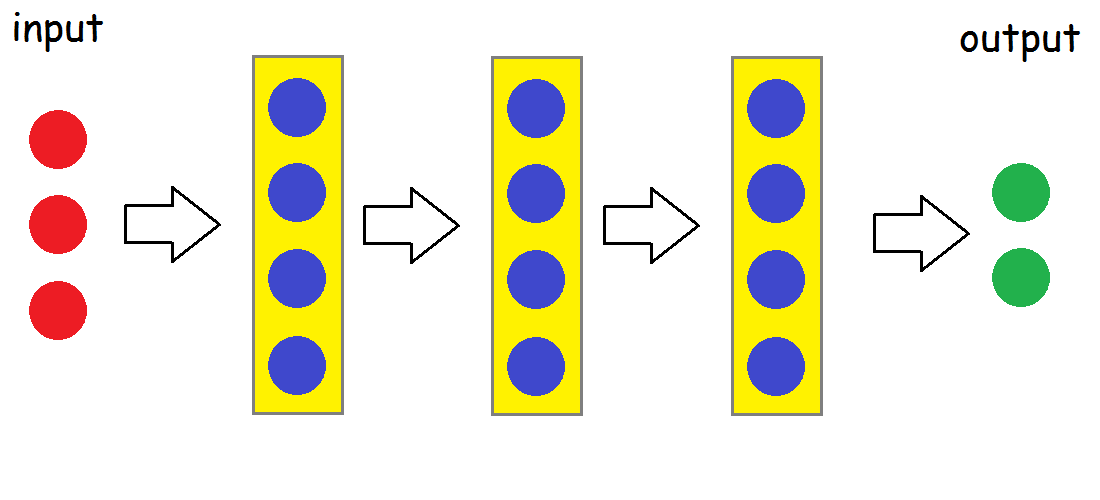
\includegraphics[width=4in]{04ANNDeep/DeepStructure.png}
\end{center}
\caption{ภาพแสดงโครงสร้างแบบลึก เปรียบเทียบกับ รูป~\ref{fig: deep shallow structure}.
  ในภาพเป็นโครงสร้างที่มี 3 ชั้นซ่อน (4-layer network).}
\label{fig: deep deep structure}
\index{deep learning}
\end{figure}
%

นอกจากมุมมองทางทฤษฎีแล้ว มุมมองจากแรงบันดาลใจของระบบธรรมชาติ ก็สนับสนุนแนวคิดของ โครงสร้างลึก.

โครงสร้างและการเชื่อมต่อ ของระบบสมองของมนุษย์ ก็มีลักษณะเป็นโครงสร้างแบบลึก.
ตัวอย่าง เช่น visual cortex \cite{NeuroscienceOnline}[Chapter 15] ที่มี สัญญาณ จากประสาทตา ผ่านไปที่ lateral geniculate nucleus (LGN).
สัญญาณจาก LGN ส่งผ่านไปที่ คอร์เทกซ์สายตา (visual cortex) ใน เขตสายตา V1 ซึ่งนับเป็นจุดเริ่มต้น การประมวลผลและรับรู้ภาพ.

นอกจากนั้น การรับรู้ของมนุษย์ ดูเหมือนจะมาจากโครงสร้างแบบลึก.
มนุษย์เรา จัดเรียงความคิดและการรับรู้ต่างๆ เป็นแบบลำดับชั้น:
เราใช้การรับรู้แบบลำดับชั้น (hierarchical perception) เช่น เรารับรู้ว่า บีเกิล เป็นพันธ์ุหมา; หมา เป็น สัตว์เลี้ยงลูกด้วยนม; และ สัตว์เลี้ยงลูกด้วยนม เป็น สิ่งมีชีวิต เป็นต้น.
มนุษย์เรา เริ่มเรียนรู้จากเรื่องง่ายๆ แล้วค่อยๆต่อยอด เพิ่มเติม เพื่อทำความเข้าใจ หรือ เพื่อ อธิบายเป็นเรื่องที่ซับซ้อนขึ้น.
วิศวกรเองก็ใช้แนวคิดของ multiple levels of abstraction ในการแตกปัญหาและวิธีแก้ เป็นปัญหาย่อยๆ.

โครงสร้างแบบลึก เป็นแนวทางหนึ่ง ที่ทำให้ เราสามารถเพิ่ม การเรียนรู้แบบเป็นลำดับชั้นนี้เข้าไปได้.
การเรียนรู้แบบเป็นลำดับชั้น เชื่อมโยงอย่างมาก กับแนวคิดของการเรียนรู้เชิงโยกย้าย และ การใช้ประโยชน์จากข้อมูลที่ไม่มีฉลาก ในงานจำแนกข้อมูล.
แนวคิด ของ การเรียนรู้เชิงโยกย้าย (transfer learning) คือ การที่เราเรียนรู้ที่จะทำงานได้ดีสำหรับงานหนึ่งแล้ว เราน่าจะเรียนรู้งานใหม่(ที่มีลักษณะใกล้เคียงกับงานเดิม)ได้ดีขึ้น.
หรือ เรียกง่ายๆว่า ใช้ประโยชน์จากพื้นความรู้เดิม เช่น การสอนการโต้คลื่น กับ คนที่ว่ายน้ำเป็นแล้ว น่าจะง่ายกว่า สอนกับคนที่ว่ายน้ำไม่เป็นเลย.
%
การใช้โครงสร้างแบบลึก ยังสามารถช่วยการทำการเรียนรู้เชิงโยกย้าย ได้อย่างมีประสิทธิภาพมากขึ้นอีกด้วย ดังอภิปรายในหัวข้อ~\ref{deep learning: self-taught learning}.

งานจำแนกข้อมูล เป็นงานการเรียนรู้แบบมีผู้สอน ซึ่ง เราต้องการตัวอย่างข้อมูล พร้อมฉลาก เพื่อฝึกโครงข่ายประสาทเทียม.
แต่ ในทางปฎิบัติแล้ว ปัญหาหลายอย่าง ข้อมูลที่มีฉลากหาได้ยาก ในขณะที่ ข้อมูลที่ไม่มีฉลาก สามารถหาได้ง่ายกว่ามาก.
ตัวอย่างเช่น งานรู้จำวัตถุ (object recognition) ซึ่งจุดประสงค์ คือ การระบุชนิดของวัตถุในภาพ.
การหาภาพทำได้ง่าย 
แต่ การหาภาพพร้อมฉลากที่ถูกต้อง ที่จะสามารถนำมาใช้ ฝึกโครงข่ายประสาทเทียมแบบมีผู้สอนนั้น ไม่ง่ายนัก.
โครงสร้างแบบลึก ยังสามารถช่วยให้เราใช้ประโยชน์ จากข้อมูลที่ไม่มีฉลาก มาเสริมการฝึกโครงข่ายประสาทเทียมแบบมีผู้สอน ได้อีกด้วย.

สรุปโดยย่อ ปัจจัยหลักๆที่ จูงใจ การใช้โครงสร้างแบบลึก มีดังนี้
\begin{itemize}
\item สามารถใช้ จำนวนรวม ของ หน่วยคำนวณ ที่น้อยกว่า โครงสร้างแบบตื้น ในการประมาณความสัมพันธ์ ที่ซับซ้อนและแปรผันสูงมาก ได้.
\item โครงสร้างทางประสาท ในธรรมชาติ มีลักษณะเป็นโครงสร้างแบบลึก.
\item โครงสร้างแบบลึก อนุญาติให้ โครงข่ายประสาทเทียม สามารถมี คุณสมบัติ hierarchical perceptions และ multiple levels of abstraction ซึ่งเป็นพื้นฐาน ของ กระบวนการคิด รับรู้ และ แก้ปัญหา ของมนุษย์ ได้.
\item โครงสร้างแบบลึก อนุญาติให้ เราสามารถใช้ ข้อมูลที่ไม่มีฉลาก (unlabeled data) มาช่วยปรับปรุง คุณภาพของการทำงานแบบมีผู้สอนได้.
ข้อมูลที่ไม่มีฉลาก สามารถหาได้ง่าย และ มีต้นทุน ต่ำกว่า การหาข้อมูลที่มีฉลาก.
\item โครงสร้างแบบลึก ยังช่วยให้การทำ การโยกย้ายการเรียนรู้ (transfer learning) ทำได้อย่างมีประสิทธิผลมากขึ้น.
\end{itemize}

ถึงแม้จะมีปัจจัยต่างๆที่ ชี้ประโยชน์ของการใช้โครงสร้างแบบลึก.
แต่อย่างไรก็ตาม การฝึกโครงสร้างแบบลึกทำได้ยากมาก จนกระทั่งช่วงปี ค.ศ. 2006 ที่ อาจารย์เจฟฟรีย์ ฮินตันและคณะ \cite{HintonEtAl2006a} เผยแพร่ ผลงานสำคัญ ที่เป็นเสมือนหลักไมล์ ของ ศาสตร์การเรียนรู้ของเครื่อง และ เป็น งานที่กระตุ้น การศึกษาวิจัย การเรียนรู้แบบลึก จนทำให้เกิดการประยุกต์ใช้อย่างกว้างขวางต่อมา.
% การศึกษาเรื่อง Deep Belief Networks (DBN) ของ เจฟฟรีย์ ฮินตัน (Geoffrey Hinton)
%\begin{itemize}
%\item Hinton, G. E., Osindero, S. and Teh, Y., A fast learning algorithm for deep belief nets, Neural Computation 18: 1527-1554, 2006.
%\item Yoshua Bengio, Pascal Lamblin, Dan Popovici and Hugo Larochelle, Greedy Layer-Wise Training of Deep Networks, in J. Platt et al (Eds), Advances in Neural Information Processing Systems 19 (NIPS 2006), pp. 153-160, MIT Press, 2007.
%\item Marc'Aurelio Ranzato, Christopher Poultney, Sumit Chopra and Yann LeCun, Efficient Learning of Sparse Representations with an Energy-Based Model, in J. Platt et al. (Eds), Advances in Neural Information Processing Systems (NIPS 2006), MIT Press, 2007.
%\end{itemize}
%

โดย อาจารย์เจฟฟรีย์ ฮินตันและคณะ \cite{HintonEtAl2006a} ใช้ Deep Belief Networks (DBNs) ที่ใช้ Restricted Boltzmann Machines (RBMs) ในการทำการเรียนรู้แบบไม่มีผู้สอน เพื่อเรียน representations ของแต่ละชั้นซ่อน;
ต่อมา ทีมของอาจารย์เบนจิโอ \cite{BengioEtAl2007a} ศึกษา และเปรียบเทียบการใช้ RBMs กับ auto-encoders;
ส่วน ทีมของอาจารย์รานซาโต \cite{RanzatoEtAl2007a} ใช้ sparse auto-encoder กับบริบทของ convolution architecture.
ทั้ง 3 แนวทาง (RBMs, autoencoders, และ convolution networks) เป็น แนวทางหลักๆ ของการศาสตร์การเรียนรู้แบบลึก ในช่วงเริ่มต้น.

หลักการที่สำคัญ ซึ่งพบในทุกๆงานเหล่านี้ ก็คือ:
\begin{itemize}
\item ใช้การเรียนรู้แบบไม่มีผู้สอน (unsupervised learning) เพื่อเรียน ลักษณะที่สำคัญ (representations) ของอินพุต ซึ่ง เท่ากับเป็น การปรับค่าน้ำหนักเริ่มต้น ให้กับ แต่ละชั้นซ่อน ของโครงสร้างแบบลึก.
\item ทำการเรียนรู้แบบไม่มีผู้สอนไปทีละชั้นซ่อน โดยเริ่มจากอินพุต ขยับไป ทางเอาต์พุต และใช้ ลักษณะสำคัญที่เรียนได้ ในแต่ละชั้น ไปใช้เป็น อินพุต สำหรับชั้นถัดไป.
ขั้นตอนการใช้ การเรียนรู้แบบไม่มีผู้สอน เพื่อช่วยหาค่าน้ำหนักเริ่มต้น แบบนี้ จะเรียกว่า การทำ พรีเทรน (pre-train).
\index{pre-train}
\item ขั้นตอนสุดท้าย คือ จะใช้การเรียนรู้แบบมีผู้สอน เพื่อ ปรับค่าน้ำหนักของทุกๆชั้นอย่างละเอียดอีกที รวมถึง การมีชั้นสุดท้าย เพิ่มขึ้นมา เพื่อให้โครงข่ายประสาทเทียม ทำงานทำนายแบบที่ต้องการ.
\end{itemize}

%รวมถึง การใช้ฟังชั่นการกระตุ้นประกอบกับเรกูลาไรเซชั่นแบบใหม่, การมีข้อมูลเป็นจำนวนมาก, และ การมีทรัพยากรคำนวณที่มีสมถนะสูง เป็น

อย่างไรก็ตาม งานศึกษาโครงสร้างแบบลึกในช่วงหลัง มีการนำเอาฟังชั่นค่ากระตุ้น ได้แก่ เรคติไฟด์ลิเนียร์ (rectified linear) \index{rectified linear} \index{เรคติไฟด์ลิเนียร์} มาใช้แทนซิกมอยด์ฟังชั่น ประกอบกับ การทำเรกูลาไรเซชั่น ด้วยวิธี ดรอปเอาต์ (dropout) \index{dropout} \index{ดรอปเอาต์} ซึ่งพบว่า ทำให้สามารถฝึกโครงข่ายได้ง่ายขึ้น.
จนกระทั่ง พบว่า หากมี ข้อมูลที่มีฉลาก เป็นจำนวนมาก, การฝึกโครงสร้างแบบลึก ก็สามารถทำได้ดี แม้ไม่ได้ทำ การปรับน้ำหนักค่าเริ่มต้นก่อน:
กล่าวคือ งานการเรียนรู้แบบลึกในช่วงหลัง พบว่า หากจำนวนข้อมูลมีมากพอ, เราสามารถใช้ โครงสร้างแบบลึก เรียนรู้งานแบบมีผู้สอนได้เลย โดย แม้แต่จะใช้ค่าน้ำหนักเริ่มต้นด้วยการสุ่ม (ไม่ต้องทำ pre-train).
นอกจากนั้น ทรัพยากรด้านการคำนวณสมถะสูง ก็เป็นอีกปัจจัยที่ทำให้การฝึกโครงข่ายแบบลึกขนาดใหญ่สามารถทำได้ดี ดังเช่น งานการจำแนกลายมือเขียน ของ ซิเรซานและคณะ \cite{CiresanEtAl2012a, MNIST20150311}.

เนื้อหาของการเรียนรู้แบบลึกต่อไปนี้ ผู้เขียนได้รับอิทธิพลหลักมาจาก 
\cite{LarochelleEtAl2007a, Larochelle2013a, Hinton2013a, Ng2012a}
โดย ผู้เขียนได้ปรับแต่งให้เหมาะสมสำหรับ การแนะนำ การเรียนรู้แบบลึก เบื้องต้น.
ผู้อ่านที่สนใจศึกษาเพิ่มเติม ผู้เขียนแนะนำแหล่งข้อมูลที่อ้างอิงเหล่านี้สำหรับการเริ่มต้น.
เพื่อให้เนื้อหา เหมาะสม สำหรับการแนะนำ การเรียนรู้แบบลึกเบื้องต้น,
ผู้เขียน แบ่งเนื้อหา ออกเป็น การเตรียมการฝึก (pre-train) และ ตัวอย่างการฝึกและประยุกต์ใช้ โครงข่ายแบบลึก
%, ตัวอย่างการใช้ฟังชั่นกระตุ้นแบบเรคติไฟด์ลิเนียร์ (rectified linear activation) และ วิธีดรอปเอาต์ (dropout).
ก่อนกระโดดไปรายละเอียด, ผู้เขียนอยากย้ำประเด็นหลักของภาพใหญ่อีกครั้ง ดังนี้:
\begin{itemize}
\item การเตรียมการฝึก (หัวข้อ~\ref{deep: pre train}): ทำเพื่อเริ่มต้นค่าน้ำหนัก ให้ดีกว่าการสุ่ม
\item ฝึกโครงข่ายแบบลึก ด้วยวิธีแพร่กระจายย้อนกลับ:
วิธีแพร่กระจายย้อนกลับ รองรับ การคำนวณของโครงข่ายแบบลึก ได้ตั้งแต่แรกแล้ว.
ไม่ได้มีอะไรเปลี่ยนแปลงจาก วิธีแพร่กระจายย้อนกลับ ที่อภิปรายกันในหัวข้อ~\ref{sec: ANN backpropagation} เลย.
เพียงให้เห็นกระบวนการทั้งหมด เราจะดูตัวอย่างสำหรับโครงข่ายแบบลึก ในหัวข้อ~\ref{deep: deep learning}.
\end{itemize}
ดังนั้น โครงข่ายแบบลึกไม่ได้มีอะไรที่ใหม่ถอดด้าม เพียงเพิ่มการเตรียมการฝึกเข้ามา และ อาจเพิ่ม เกร็ดเล็กๆน้อยๆ บางอย่าง เข้ามาเท่านั้น.
เกร็ดเล็กๆน้อยๆ นั้น รวมถึง การใช้ ฟังชั่นกระตุ้นแบบเรคติไฟด์ลิเนียร์ (rectified linear activation)\cite{HintonBrainSexML}, การทำเรกูลาไรเซชั่น ด้วย วิธีดรอปเอาต์\cite{DahlSainathHinton2013a}, การเลือกใช้ convolution layer\cite{CouprieEtAl2014a} สำหรับ อินพุตที่มิติมีความเกี่ยวพันกัน, การทำ mini-batch\cite{HintonRecipe} เป็นต้น.
สำหรับเกร็ดเล็กๆน้อยๆ ต่างๆ ผู้เขียนแนะนำ ให้ดู \cite{HintonRecipe} สำหรับรายละเอียดและคำแนะนำในทางปฎิบัติ.
 %หากอินพุตมีลักษณะที่มิติสัมพันธ์กันเชิงตำแหน่ง

\subsection{การเตรียมการฝึก}
\label{deep: pre train}
\index{การเตรียมการฝึก}
\index{pre-train}

การเตรียมการฝึก คือ การกำหนด ค่าเริ่มต้นให้กับ ค่าน้ำหนัก.
จากบท~\ref{chapter: Applications of ANN}, เราอภิปราย เรื่อง การกำหนดค่าเริ่มต้นให้กับ ค่าน้ำหนัก ของโครงข่ายประสาทเทียมด้วยการสุ่ม.
ถ้าโครงข่ายของเราตื้น หรือ ว่าเรามีข้อมูลมากพอ, การกำหนดค่าเริ่มต้นให้กับ ค่าน้ำหนัก ด้วยการสุ่มก็ทำงานได้ดี.

แต่หากเราไม่ได้มีข้อมูลมากพอ และ เราใช้โครงข่ายที่ลึก, ในทางปฏิบัติแล้ว การฝึกโครงข่ายประสาทเทียมแบบลึก ในปัญหาที่ซับซ้อน จะทำได้ยากมาก ถ้าเริ่มต้น ค่าน้ำหนัก ด้วยการสุ่ม.
แทนการสุ่มค่า, การเตรียมการฝึก (pre-training) จะใช้แนวทางของการเรียนรู้แบบไม่มีผู้สอน (unsupervised learning) เพื่อช่วย การกำหนดค่าเริ่มต้นให้กับ ค่าน้ำหนัก.
ในการเตรียมการฝึก เราจะใช้แค่อินพุต $\mathbf{x}_n$.
เรายังไม่ใช้เอาต์พุต (ฉลาก หรือ เฉลย), ดังนั้น แนวทางนี้ช่วยให้เราสามารถใช้ประโยชน์ จากข้อมูลที่ไม่มีฉลากได้ดีขึ้น.
แนวคิด คือ เราจะใช้ ตัวอย่าง อินพุต $\mathbf{x}_n$
 เพื่อฝึกโครงข่ายให้ คัดเลือก ลักษณะสำคัญ ของตัวอย่างอินพุต เหล่านั้นออกมา.
โดย เราจะใช้แนวทางของเรกูลาไรเซชั่น เพื่อบังคับให้โครงข่าย คัดเลือก ลักษณะสำคัญ ออกมา, แทนที่จะ แค่ทำอะไรทึ่มๆ\footnote{
ดู กรอบ ตัวอย่างโอเวอร์ฟิต.
} ออกมา.

\subsubsection{ออโตเอนโค้ดเดอร์}
\label{deep: autoencoder}
วิธีหนึ่ง ที่สามารถใช้เตรียมค่าน้ำหนักเริ่มต้นได้ดี คือ ออโตเอนโค้ดเดอร์ (autoencoder) \index{Autoencoder} \index{ออโตเอนโค้ดเดอร์}.
ออโตเอนโค้ดเดอร์ เป็น โครงข่ายประสาทเทียมแบบจ่ายไปข้างหน้าขนาด $2$ ชั้น (2-layer feed forward neural network), ซึ่งคือ โครงข่าย แบบเดียวกับที่อภิปรายมาตลอด ในบท~\ref{chapter: ANN}, \ref{chapter: Applications of ANN}, และ \ref{chapter: Suggestions for ANN};
เพียงแต่ เราฝึกให้ โครงข่ายพยายามเลียนแบบ ตัวอย่างอินพุต.
กล่าวคือ, มีอินพุต $\mathbf{x}$, ฝึกโครงข่าย ให้พยายามเลียนแบบ เพื่อให้เอาต์พุต $\hat{\mathbf{x}}$ ใกล้เคียงกับ $\mathbf{x}$ มากที่สุด.
การทำเช่นนี้ สอดคล้องกับ ชื่อ ``autoencoder'' ที่สื่อถึง การนำตัวเองไปเข้ารหัส.

%
\begin{figure}
\begin{center}
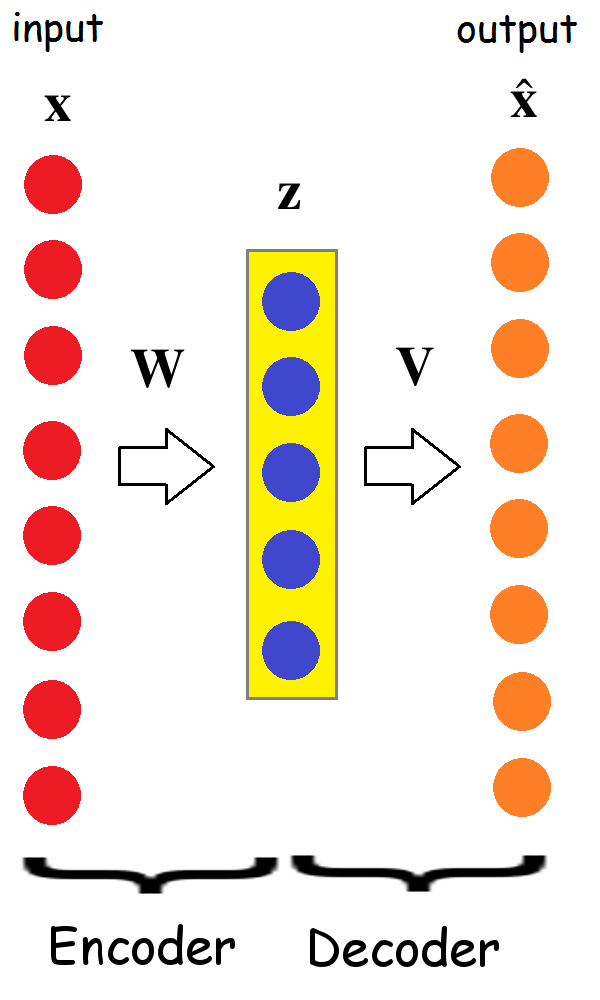
\includegraphics[width=2in]{04ANNDeep/Autoencoder.png}
\end{center}
\caption{ออโตเอนโค้ดเดอร์ พยายามเลียนแบบอินพุต: พยายามปรับค่าน้ำหนัก $\mathbf{W}$ และ $\mathbf{V}$ เพื่อให้ $\hat{\mathbf{x}}$ คล้าย $\mathbf{x}$ ที่สุด;
หากเราสามารถควบคุมกระบวนการไม่ให้เกิดโอเวอร์ฟิตได้, เราน่าจะได้ลักษณะสำคัญของอินพุตออกมา}
\label{fig: deep autoencoder}
\end{figure}
%

รูป~\ref{fig: deep autoencoder} แสดงออโตเอนโค้ดเดอร์.
เราฝึกโครงข่ายนี้ เพื่อหาค่าน้ำหนัก ที่ทำให้เอาต์พุต $\hat{\mathbf{x}}$ คล้าย อินพุต $\mathbf{x}$ มากที่สุด;
หากเราสามารถควบคุมไม่ให้เกิดโอเวอร์ฟิตได้, เราน่าจะได้ ค่าน้ำหนักที่เชื่อมโยงกับลักษณะสำคัญของอินพุต ออกมาได้;
และ ค่าน้ำหนักที่เชื่อมโยงกับลักษณะสำคัญของอินพุต น่าจะเป็นค่าน้ำหนักที่ดี สำหรับ ใช้ต่อไปเพื่อทำงานที่ต้องการ เช่น การจำแนกกลุ่ม หรือ การหาค่าถดถอย เป็นต้น.

\begin{minipage}{5.5in}
{\small
\begin{shaded}
\underline{\textbf{ตัวอย่าง โอเวอร์ฟิต}} ในบริบทนี้ เช่น การมีจำนวนหน่วยซ่อน เท่ากับ จำนวนอินพุต และ หากเราไม่ควบคุมอะไรเลย เราอาจได้ค่าน้ำหนักที่ทำให้เกิด one-to-one mapping ระหว่างอินพุต $\mathbf{x}$ และ $\mathbf{z}$ และ ระหว่าง $\mathbf{z}$ และ $\hat{\mathbf{x}}$,
ซึ่งทำให้ $\hat{\mathbf{x}} = \mathbf{x}$ อย่างสมบูรณ์;
แต่ เรา ไม่ได้ ลักษณะสำคัญ (features) อะไรเลย และ ค่าน้ำหนักที่ได้ก็ไม่ได้มีประโยชน์อะไรเลย.
เราจะอภิปรายรายละเอียด เรื่อง วิธีการควบคุมที่ว่านี้ ต่อไป.

\end{shaded}
}%small
\end{minipage}

ก่อนอื่น ผู้เขียนชี้แจงประเด็นหนึ่งที่มักจะทำให้สับสน คือ สิ่งที่เราทำอยู่, เราไม่ได้หาสิ่งที่เราอยากได้ตรงๆ.
สิ่งที่เราต้องการในกระบวนการเตรียมการฝึกนี้ คือ ค่าน้ำหนักเริ่มต้นที่ดี.
เราหา ค่าน้ำหนักเริ่มต้นที่ดี โดยเชื่อว่า ค่าน้ำหนักเริ่มต้นที่ดี คือ ค่าน้ำหนักที่เชื่อมโยงกับลักษณะสำคัญของอินพุต.
และ เราหา ค่าน้ำหนักที่เชื่อมโยงกับลักษณะสำคัญ โดยวิธีอ้อม, 
ซึ่งคือ สำหรับออโตเอนโค้ดเดอร์ คือ การหาค่าน้ำหนัก ที่ทำให้ โครงข่ายเลียนแบบอินพุตได้ดีที่สุด.

กลับไปที่รูป~\ref{fig: deep autoencoder}, นี้คือ โครงข่ายประสาทเทียม $2$ ชั้นธรรมดา, 
เพียงเราจัดตัวอย่างฉลากให้เป็นอินพุต.
ส่วนหน้าของออโตเอนโค้ดเดอร์ (โครงข่ายชั้นแรก), ค่าเอาต์พุตของชั้นที่หนึ่ง (ชั้นซ่อน),
\begin{eqnarray}
\mathbf{a} &=& \mathbf{W} \cdot \mathbf{x}
\label{eq: deep autoencoder a} \\
\mathbf{z} &=& \mathrm{sigmoid}(\mathbf{a})
\label{eq: deep autoencoder z}
\end{eqnarray}
เมื่อ $\mathbf{x}$ เป็นอินพุตเวกเตอร์ ขนาด $D$ มิติ,
$\mathbf{W}$ เป็นเมตริกซ์ของน้ำหนักชั้นที่หนึ่ง ขนาด $M \times (1+D)$ 
สำหรับโครงข่ายที่มี $M$ หน่วยซ่อน,
$\mathbf{a}$ เป็นเวกเตอร์แทนค่าการกระตุ้น,
และ $\mathbf{z}$ เป็นเวกเตอร์ของเอาต์พุตชั้นซ่อน, ซึ่งคือ ค่าการกระตุ้น ที่ผ่านซิกมอยด์ฟังชั่น.

หากทำออโตเอนโค้ดเดอร์ได้อย่างดีแล้ว, ค่าเอาต์พุตของชั้นซ่อน $\mathbf{z}$ จะทำหน้าที่เสมือนเป็น ตัวตรวจจับลักษณะสำคัญ (feature detector).
เช่น มีอินพุต $\mathbf{x}_n$, แล้ว ค่าเอาต์พุตของชั้นซ่อน ตัวที่ $5$ กับ $8$ มีใกล้ๆ $1$ ในขณะตัวอื่นๆมีค่าใกล้ๆ $0$, เราอาจบอกได้ว่า อินพุต $\mathbf{x}_n$ นี้ มีลักษณะสำคัญ $2$ อย่าง: บ่งบอกด้วย หน่วยซ่อนตัวที่ $5$ และ $8$.
ชั้นแรกนี้ จะทำหน้าที่เสมือนการเข้ารหัสอินพุตไว้ เป็นลักษณะสำคัญ, เราเรียกชั้นนี้ว่า ตัวเข้ารหัส หรือ ``Encoder''.

ส่วนหลังของออโตเอนโค้ดเดอร์ (โครงข่ายชั้นสอง), ค่าเอาต์พุต,
\begin{eqnarray}
\hat{\mathbf{a}} &=& \mathbf{V} \cdot \mathbf{z}
\label{eq: deep autoencoder a hat} \\
\hat{\mathbf{x}} &=& \mathrm{sigmoid}(\hat{\mathbf{a}})
\label{eq: deep autoencoder x hat}
\end{eqnarray}
เมื่อ $\mathbf{V}$ เป็น เมตริกซ์ค่าน้ำหนักของชั้นที่สอง ขนาด $D \times (1+M)$,
$\hat{\mathbf{a}}$ เป็น เวกเตอร์ค่ากระตุ้นของชั้นที่สอง,
และ $\hat{\mathbf{x}}$ คือ เอาต์พุตของออโตเอนโค้ดเดอร์.
หมายเหตุ สมการ~\ref{eq: deep autoencoder x hat} ใช้ ฟังชั่นกระตุ้นเป็นซิกมอยด์ฟังชั่น ซึ่งเหมาะสมกับ กรณีที่อินพุตเป็นลักษณะฐานสอง\footnote{
เทียบเท่ากับ งานจำแนกกลุ่มแบบ $2$ กลุ่ม (biclass classification): ฟังชั่นกระตุ้นชั้นเอาต์พุต ที่เหมาะสม คือ ซิกมอยด์ฟังชั่น (sigmoid): $f(a) = \frac{1}{1+\exp(-a)}$.
ในขณะที่ อินพุตที่เป็นลักษณะค่าต่อเนื่อง ซึ่งเทียบเท่ากับงานหาค่าถดถอย (regression),
ฟังชั่นกระตุ้นชั้นเอาต์พุต ที่เหมาะสม คือ ฟังชั่นอัตลักษณ์ (identity): $f(a) = a$.
%
ดูตาราง~\ref{tbl: ANN output activation function} ประกอบ.
} (มีค่า $0$ หรือ $1$)

การทำงานของส่วนหลังของออโตเอนโค้ดเดอร์ จะทำหน้าที่ แปลง ลักษณะสำคัญ กลับไป ให้คล้าย อินพุต, เรียกว่า ตัวถอดรหัส หรือ ``Decoder''.
ทบทวนภาพรวม, ในการทำออโตเอนโค้ดเดอร์ เราถ้าหาค่าน้ำหนักทั้งส่วนหน้า (ตัวเข้ารหัส) $\mathbf{W}$ และ ส่วนหลัง (ตัวถอดรหัส) $\mathbf{V}$. แต่หลังจากเสร็จกระบวนการเตรียมการฝึกแล้ว สิ่งที่เราได้ไปใช้ต่อจริง จะมีแค่ ค่าน้ำหนักของส่วนหน้า คือ $\mathbf{W}$ เท่านั้น, เราจะไม่ได้ใช้ $\mathbf{V}$ อีก.
หัวข้อ~\ref{deep: deep learning} จะให้ตัวอย่าง ของทั้งกระบวนการตั้งแต่แรก จนเสร็จ.

ในทางปฎิบัติ มีความนิยมที่กำหนดให้
\begin{eqnarray}
\mathbf{\dot{V}} = \mathbf{\dot{W}}^T
\label{eq: deep tied weight}
\end{eqnarray}
โดย $\mathbf{\dot{V}}$ แทน เมตริกซ์ของค่าน้ำหนักของออโตเอนโค้ดเดอร์ส่วนหลัง โดยไม่รวมไบอัส ดังนั้นขนาด $[D \times M]$
และ $\mathbf{\dot{W}}$ แทน เมตริกซ์ของค่าน้ำหนักของออโตเอนโค้ดเดอร์ส่วนหน้า โดยไม่รวมไบอัสเช่นเดียวกัน, ขนาด $[M \times D]$.
การทำเช่นนี้ จะเรียกว่า ``tied weight'', 
เหตุผลเบื้องหลัง นอกจากลดการคำนวณลงแล้ว ยังทำให้การทำงานของออโตเอนโค้ดเดอร์ คล้ายคลึงกับ Restricted Boltzmann Machines ที่เป็นเสมือนหลักไมล์ของการเรียนรู้แบบลึกด้วย.

\paragraph{ขนาดของชั้นซ่อนในออโตเอนโค้ดเดอร์.}
% Larochelle's lecture
หาก จำนวนหน่วยซ่อนในออโตเอนโค้ดเดอร์ มีน้อยกว่า มิติของอินพุต, ดังแสดงในรูป~\ref{fig: deep autoencoder},
เราจะเรียกว่า undercomplete hidden layer.
เมื่อเราฝึกให้ ออโตเอนโค้ดเดอร์ เลียนแบบอินพุต ก็เทียบเท่ากับว่า เราบังคับให้ ออโตเอนโค้ดเดอร์ พยายามหา ``รูปแบบการบีบอัด'' ของอินพุต.
การบีบอัด (compression) อาจช่วยให้เราได้ลักษณะที่สำคัญของอินพุตตัวอย่าง
ซึ่งเราอาจได้ การบีบอัด ที่ดีสำหรับตัวอย่างที่นำมาฝึก, แต่ก็อาจจะไม่เพียงพอสำหรับอินพุตทั่วๆไป.

%Undercomplete hidden layer is undercomplete if it is smaller than the input layer
%* compress the input
%* compress well only for the training distribution
%Hidden units will be 
%* good features for the training distribution
%* but bad for other types of input

หากจำนวนหน่วยซ่อนในออโตเอนโค้ดเดอร์ มีมากกว่า มิติของอินพุต, ดังแสดงในรูป~{fig: deep overcomplete hidden layer},
เราเรียกว่า ``overcomplete hidden layer''.
กรณีนี้ไม่มีการบีบอัดข้อมูลในชั้นซ่อน.
มีความเสี่ยงที่ หน่วยซ่อนจะ ไม่ได้จับลักษณะสำคัญ ไม่ได้จับโครงสร้างอะไรที่มีความหมาย ออกมา, 
หน่วยซ่อนอาจจะแค่ คัดลอกค่ามาจากอินพุต ดังที่ได้อภิปรายในกรอบ\underline{\textbf{ตัวอย่าง โอเวอร์ฟิต}}.

%Overcomplete hidden layer is overcomplete if it is greater than the input layer
%* no compression in hidden layer
%& each hidden unit could copy a different input component

%No guarantee that the hidden units will extract meaningful structure.

%
\begin{figure}
\begin{center}
\includegraphics[width=2in]{04ANNDeep/overcomplete.png}
\end{center}
\caption{ออโตเอนโค้ดเดอร์ที่ชั้นซ่อนมีขนาดใหญ่กว่าอินพุต: หากไม่มีการควบคุมใดๆ เราไม่สามารถรับประกันได้ว่า การฝึกออโตเอนโค้ดเดอร์จะได้ ลักษณะสำคัญ ที่มีประโยชน์ออกมา.}
\label{fig: deep overcomplete hidden layer}
\end{figure}
%

หากเราต้องการจำนวนหน่วยซ่อนที่มาก เพื่อเพิ่มความยืดหยุ่นของโมเดล\footnote{
การใช้จำนวนหน่วยซ่อนที่มาก สัมพันธ์ กับ การลดไบอัส.
ในขณะที่ การควบคุม ไม่ให้ จำนวนหน่วยซ่อนที่มาก นำไปสู่ โครงข่ายทึ่มๆ สัมพันธ์ กับ การลดความแปรผัน.
ทบทวนหัวข้อ~\ref{ann tips: bias v.s. variance} สำหรับ การวิเคราะห์ความผิดพลาดของโมเดล และ ความสัมพันธ์ระหว่าง ความซับซ้อนของโมเดล กับ ไบอัส และ ความแปรผัน.
} แต่ต้องการควบคุมไม่ให้ได้โครงข่ายทึ่มๆออกมา,
เราสามารถทำได้หลายวิธี, หนึ่งในนั้น คือ วิธี ดินอยซิ่ง (denoising).

``One of the main purposes of unsupervised learning is to produce good representation for data, that can be used for detection, recognition, prediction, or visualization. 
Good representation eliminate irrelevant variabilities of the input data, 
while preserving the information that is useful for the ultimate task.''
Marc'Aurelio Ranzato, Y-Lan Boureau and Yann LeCun\cite{RanzatoEtAl2007b}

\paragraph{Denoising Autoencoder.} \index{denoising autoencoder} \index{ดินอยซิ่งออโตเอนโค้ดเดอร์}
แนวคิด คือ การทำงานของโครงข่าย น่าจะสามารถทนทานต่อ สัญญาณรบกวน ได้ดีระดับหนึ่ง.
วิธีของ ดินอยซิ่งออโตเอนโค้ดเดอร์ (denoising autoencoder) คือ จะใส่ สัญญาณรบกวน เข้าไปในอินพุตตัวอย่าง.
เช่น สำหรับอินพุตที่มีลักษณะเป็นไบนารี่ (binary input) อาจจะสุ่มเลือกอินพุตบางมิติออกมาแล้วให้ค่าเป็น $0$ ตามความน่าจะเป็นที่ระบุ
หรือ สำหรับ อินพุตที่เป็นลักษณะค่าต่อเนื่อง อาจจะเพิ่มสัญญาณรบกวนแบบเกาส์เชี่ยนเข้าไป เป็นต้น.

%representation น่าจะ robust 
%* idea: representation should be robust to introduction of noise.
%** random assignment of subset of inputs to $0$ with probability $\nu$ (maybe for binary input)
%** We can do other type, e.g., Gaussian additive noise (maybe for continuous input)

%
\begin{figure}
\begin{center}
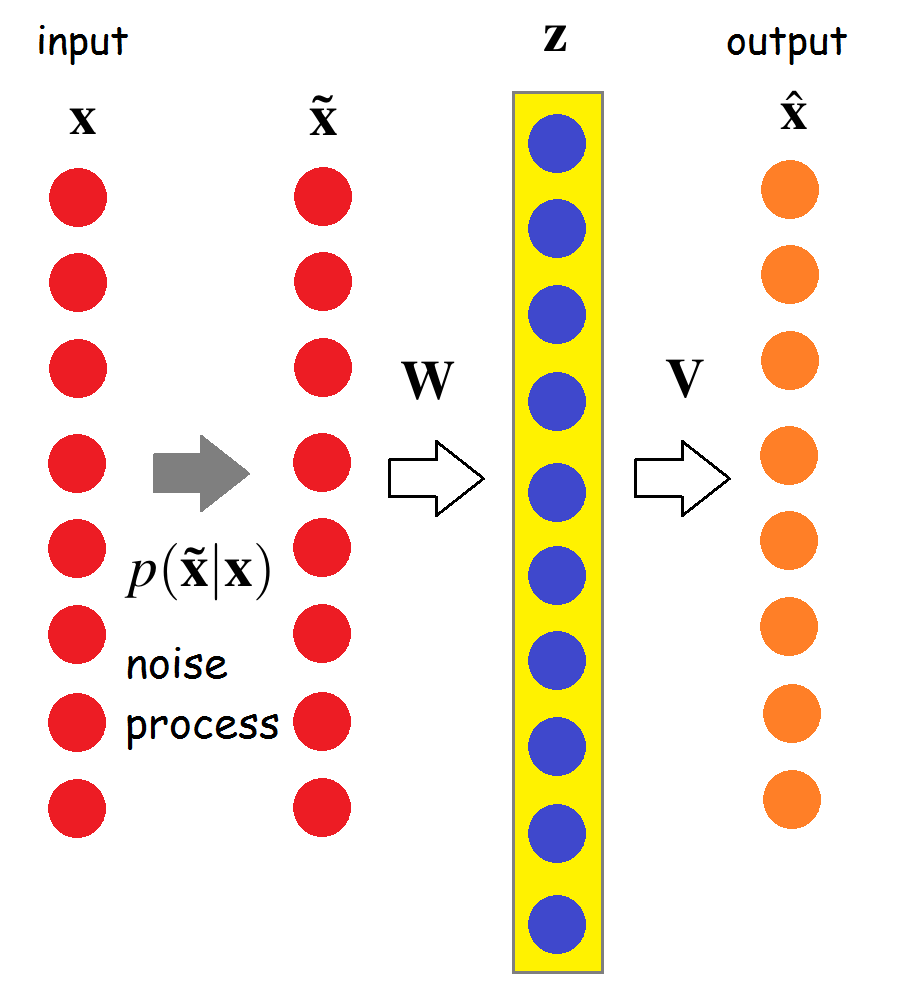
\includegraphics[width=2.5in]{04ANNDeep/denoisingAutoencoder.png}
\end{center}
\caption{ดินอยซิ่งออโตเอนโค้ดเดอร์(denoising autoencoder): ทำด้วยการใส่สัญญาณรบกวนเข้าไปในอินพุต.}
\label{fig: deep denoising autoencoder}
\end{figure}
%

รูป~\ref{fig: deep denoising autoencoder} แสดง โครงสร้างของ ดินอยซิ่งออโตเอนโค้ดเดอร์.
จากอินพุตตัวอย่าง $\mathbf{x}$, เราจะใส่สัญญาณรบกวนเข้าไป.
อินพุตที่รวมกับสัญญาณรบกวน, $\mathbf{\tilde{x}}$, จะใช้เป็น ตัวอย่างเพื่อฝึกออโตเอนโค้ดเดอร์.
ออโตเอนโค้ดเดอร์ จะพยายามสร้าง $\hat{\mathbf{x}}$ ขึ้นมาจาก อินพุตที่ถูกรบกวน $\mathbf{\tilde{x}}$.
แต่ ฟังชั่นเป้าหมาย (objective function) เปรียบเทียบ $\hat{\mathbf{x}}$ กับ อินพุตต้นฉบับ $\mathbf{x}$.
หรือ พูดอีกนัยหนึ่ง, เราใส่ อินพุตที่เสียหายเข้าไป แต่พยายามฝึกโครงข่ายให้ทายว่า อินพุตที่สมบูรณ์หน้าตาเป็นอย่างไร.

การทำแบบนี้ ทำให้ แม้เราจะเลือกใช้ overcomplete hidden layer (จำนวนหน่วยซ่อนมากกว่ามิติของอินพุต), แต่ ความเสี่ยงที่เราจะได้โครงข่ายทึ่มๆออกมา จะน้อยมาก;
เพราะว่า หน่วยซ่อน จะคัดลอกอินพุต แล้วผ่านต่อไปเป็นเอาต์พุต ไม่ได้:
อินพุตที่โครงข่ายเห็นเป็นอินพุตที่เสียหายจากสัญญาณรบกวน เมื่อไปเปรียบเทียบกับ เฉลย ซึ่งเป็นอินพุตจริงที่ไม่มีสัญญาณรบกวน จะต่างกันมาก.
ดังนั้น การทำดินอยซิ่ง เป็น การบังคับให้ออโตเอนโค้ดเดอร์ ต้องหา ลักษณะอื่น จากอินพุตที่เสียหาย เพื่อ ซ่อมแซมให้กลับไปเป็นอินพุตต้นฉบับ.

%* Reconstruction $\hat{\mathbf{x}}$ computed from the corrupted input $\tilde{\mathbf{x}}$

%* Loss function compare $\hat{\mathbf{x}}$ reconstruction with the noiseless input $\mathbf{x}$.

%You can't just copy noisy input to hidden units, because it couldn't compare well with noiseless input.
%Autoencoder will be forced to use other input to guess or fix damaged input.

%
\begin{figure}
\begin{center}
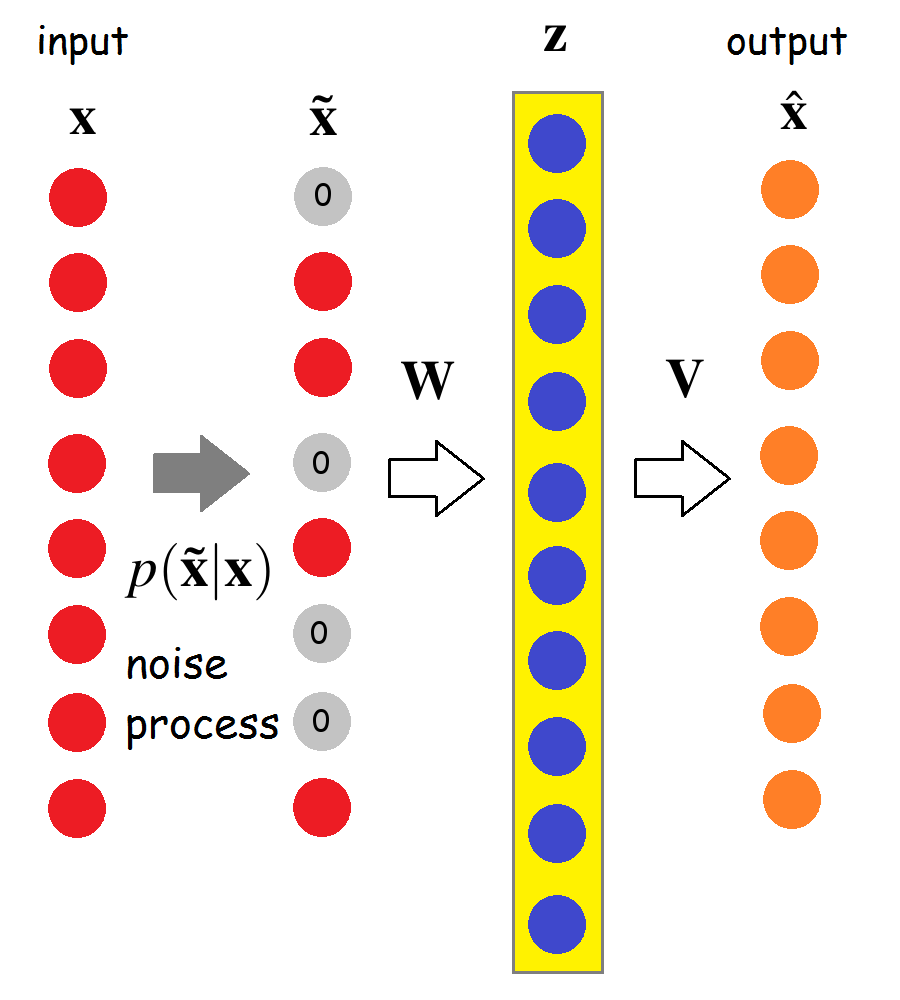
\includegraphics[width=2.5in]{04ANNDeep/binaryDenoisingAutoencoder.png}
\end{center}
\caption{แสดง ดินอยซิ่งออโตเอนโค้ดเดอร์(denoising autoencoder) เมื่อ สุ่มอินพุตออก.
เราอาจสุ่มให้อินพุตบางมิติเป็น $0$ ตามความน่าจะเป็นที่เรากำหนดได้.
ในรูป อินพุตมิติ 2, 3, 5, และ 8 (นับจากล่างขึ้นบน) ถูกสุ่มให้เป็น $0$ สำหรับจุดข้อมูลตัวอย่างนั้น; สำหรับจุดข้อมูลตัวอย่างใหม่ เราก็จะสุ่มใหม่.}
\label{fig: deep binary denoising autoencoder}
\end{figure}
%

อีกมุมหนึ่ง อาจมองว่า การใส่สัญญาณรบกวน เข้าไป เป็นการเพิ่มความแปรผันของตัวอย่าง เพิ่มความหลากหลายของตัวอย่าง.
ดังนี้จะ ช่วยให้โมเดลเห็น ลักษณะสำคัญ ของตัวอย่างได้ดีขึ้น ในแง่ที่ว่า สัญญาณรบกวน รบกวนแค่รายละเอียดปลีกย่อย แต่ลักษณะสำคัญ ที่เป็นภาพใหญ่ยังคงอยู่.
ดังนั้น แม้จะฟังดูแปลกๆที่ เราใส่สัญญาณรบกวนเข้าไป เพื่อดึงลักษณะสำคัญ ออกมา, แต่ การกวนลักษณะปลีกย่อย จะทำให้ ลักษณะสำคัญ เด่นชัดขึ้น เพราะ 
ปริมาณสัญญาณรบกวนที่ใส่เข้าไป ไม่มากพอจะกวน ลักษณะสำคัญ แต่พอที่จะเข้าไปกวน ลักษณะปลีกย่อย.
ลองนึกถึง ภาพถ่ายของ ชนพื้นเมืองอเมริกา,
หากภาพตัวอย่าง มี ภาพชนพื้นเมืองที่อยู่บ้านสมัยปัจจุบัน, ภาพชนพื้นเมืองที่อยู่กระโจม, 
ภาพชนพื้นเมืองที่อยู่บ้านดินเหนียว, ภาพชนพื้นเมืองที่แต่งกายด้วยชุดพื้นเมือง, ภาพชนพื้นเมืองที่แต่งกายด้วยเสื้อผ้าทั่วไป, ภาพชนพื้นเมืองขับรถ, ภาพชนพื้นเมืองขี่ม้า,
เราก็จะบอกลักษณะได้ว่า ชนพื้นเมือง มีลักษณะเด่น อย่างไร เช่น ลักษณะเด่นของโครงหน้า.
แต่หาก ภาพตัวอย่าง มีแต่ ภาพชนพื้นเมืองที่อยู่กระโจม, กระโจมเล็กบ้าง ใหญ่บ้าง มีลวดลายมากบ้าง น้อยบ้าง, บางคนอาจเข้าใจลักษณะสำคัญผิด ไปว่า ชนพื้นเมืองต้องอยู่กระโจม.

\begin{minipage}{5.5in}
{\small
\begin{shaded}
การเพิ่มความแปรผันของตัวอย่าง เพิ่มความหลากหลายของตัวอย่าง เป็น เทคนิคทั่วไป ที่มักนำมาใช้ช่วยการฝึกโครงข่ายประสาทเทียม อยู่แล้ว.
ดังที่
อาจารย์ ไซมอน เฮย์กิน แนะนำ %เพื่อช่วยให้ อัลกอริทึ่มแพร่กระจายย้อนกลับ ทำงานได้ดีขึ้น เช่น 
ให้พยายามทำ
 ข้อมูลตัวอย่าง (ที่ใช้ฝึก) มีความหลากหลาย จากมุมมองของงานที่ทำให้มากที่สุด.

``As a general rule, every training example presented to the backpropagation algorithm should be chosen on the basis that its information content is the largest possible for the task at hand.''
- Simon Haykin\cite[pp. 175]{Haykin2009a}

ดังนั้น สิ่งที่เราอาจจะทำได้ คือ
\begin{itemize}
\item เลือกใช้ ตัวอย่าง ที่ให้ ค่าผิดพลาดของการฝึก (training error) สูง;
\item เลือกใช้ ตัวอย่าง ที่แตกต่างอย่างชัดเจน จากตัวอย่างที่ผ่านๆมา;
\end{itemize}
เชื่อว่า การทำเช่นนี้ เชื่อว่า จะช่วยให้ อัลกอริทึ่มแพร่กระจายย้อนกลับ สามารถค้นหาค่าน้ำหนัก จาก weight space ได้ทั่วถึงมากขึ้น.
\end{shaded}
}%small
\end{minipage}

\subsubsection{ออโตเอนโค้ดเดอร์ เพื่อ เตรียมการฝึกโครงข่ายแบบลึก}
\label{deep: stacked autoencoder}
% Larochelle Lecture 7.3

หัวข้อ~\ref{deep: autoencoder} เราดูวิธีทำออโตเอนโค้ดเดอร์ มาแล้ว.
การนำ ออโตเอนโค้ดเดอร์ มาใช้ หาค่าน้ำหนักเริ่มต้น ให้กับโครงข่ายแบบลึก โดยจะทำทีละชั้น (layer-wise procedure), ดังแสดงในรูป~\ref{fig: deep layer-wise pretrain}.
รูป~\ref{fig: deep autoencoder L1} เราหาค่า $\mathbf{W}^{(1)}$ ได้จาก ดินอยซิ่งออโตเอนโค้ดเดอร์\footnote{
มีวิธีอื่นๆที่ใช้ หาค่าน้ำหนักเริ่มต้น ได้นอกจาก ดินอยซิ่งออโตเอนโค้ดเดอร์\cite{VicentEtAl2008a}, เช่น Restricted Bolzman Machine\cite{HintonEtAl2006a}, 
%Staked Autoencoder\cite{BengioEtAl2007a}, 
Sparse Autoencoder\cite{RanzatoEtAl2007a},
Stacked Semi-Supervised Embeddings\cite{WestonEtAl2008a},
Stacked kernal PCA\cite{ChoSaul2009a},
และ
Stacked Independent Subspace Analysis\cite{LeEtAl2011a} เป็นต้น.

แต่เพื่อความกระชับ เราจะใช้ ดินอยซิ่งออโตเอนโค้ดเดอร์ เป็นเสมือนตัวแทน ของ เทคนิคเหล่านี้ ที่ใช้การเรียนรู้แบบไม่มีผู้สอน มาช่วยหาค่าน้ำหนักเริ่มต้น โดยทำทีละชั้น.
}%
: ใส่สัญญาณรบกวนเข้าไปในอินพุต $\mathbf{x}$ ได้เป็น อินพุตกวนๆ (noisy input) $\mathbf{\tilde{x}}$,
ใช้ฝึก %(ปรับค่าน้ำหนัก $\mathbf{W}$, สมการ~\ref{eq: deep autoencoder a hat}) 
ดินอยซิ่งออโตเอนโค้ดเดอร์ ให้ทายอินพุตต้นฉบับ $\mathbf{x}$ จาก อินพุตกวนๆ $\mathbf{\tilde{x}}$.
เราจะได้ค่าน้ำหนักส่วนหน้าของดินอยซิ่งออโตเอนโค้ดเดอร์ออกมา ($\mathbf{W}$ ที่แสดงในรูป~\ref{fig: deep denoising autoencoder} ประกอบ).

เมื่อเสร็จชั้นที่หนึ่งแล้ว, เราก็ใช้ค่า $\mathbf{W}^{(1)}$ ที่ได้มาคำนวณหา อินพุต สำหรับ ชั้นที่สอง, $\mathbf{x}^{(2)} = \mathbf{z}^{(1)} = h^{(1)}(\mathbf{W}^{(1)} \cdot \mathbf{z}^{(0)}) = h^{(1)}(\mathbf{W}^{(1)} \cdot \mathbf{x})$.
เราใช้ ค่า $\mathbf{z}^{(1)}$ เป็น อินพุตของดินอยซิ่งออโตเอนโค้ดเดอร์ เพื่อ ค่าน้ำหนักส่วนหน้าของดินอยซิ่งออโตเอนโค้ดเดอร์ออกมา, และค่าน้ำหนักที่หาได้นี้ ก็จะใช้เป็นค่าเริ่มต้นของ $\mathbf{x}^{(2)}$.
ดู รูป~\ref{fig: deep autoencoder L2} ประกอบ.

เช่นเดียวกัน เราก็ใช้ $\mathbf{W}^{(1)}$ และ $\mathbf{W}^{(2)}$ เพื่อคำนวณหา $\mathbf{z}^{(2)}$ ได้.
และ ค่า $\mathbf{z}^{(2)}$ ก็จะใช้เป็น อินพุตของดินอยซิ่งออโตเอนโค้ดเดอร์ เพื่อหา $\mathbf{W}^{(3)}$ ต่อไป (รูป~\ref{fig: deep autoencoder L3}).
เช่นเดียวกับ ชั้นที่ลึกๆขึ้นไป (รูป~\ref{fig: deep autoencoder L4}).

\begin{figure}
\centering
\begin{subfigure}[b]{\textwidth}
\includegraphics[height=1.8in]{04ANNDeep/PreTrainDeepL1.png}
\caption{ออโตเอนโค้ดเดอร์ หา $\mathbf{W}^{(1)}$: ใช้อินพุตของโครงข่าย $\mathbf{x}$ เป็นอินพุตของออโตเอนโค้ดเดอร์ ฝึก ออโตเอนโค้ดเดอร์ เพื่อเลียนแบบ $\mathbf{x}$.
ค่าน้ำหนักส่วนหน้าของออโตเอนโค้ดเดอร์ที่ได้ คือ ค่าน้ำหนักชั้นที่ต้องการ: $\mathbf{W}^{(1)} = $ W, เมื่อ W คือ ค่าน้ำหนักส่วนหน้าของออโตเอนโค้ดเดอร์ หลังจากฝึกออโตเอนโค้ดเดอร์เสร็จ.
}
\label{fig: deep autoencoder L1}
\end{subfigure}%

%~ add desired spacing between images, e. g. ~, \quad, \qquad etc.
%(or a blank line to force the subfigure onto a new line)
\begin{subfigure}[b]{\textwidth}
\includegraphics[height=1.8in]{04ANNDeep/PreTrainDeepL2.png}
\caption{จากค่า $\mathbf{W}^{(1)}$ ที่ได้, คำนวณหาค่า $\mathbf{z}^{(1)}$ ของแต่ละ $\mathbf{x}$, แล้วใช้ $\mathbf{z}^{(1)}$ เป็นอินพุตของออโตเอนโค้ดเดอร์
และ $\mathbf{W}^{(2)}  = $ W.
}
\label{fig: deep autoencoder L2}
\end{subfigure}%

%~ add desired spacing between images, e. g. ~, \quad, \qquad etc.
%(or a blank line to force the subfigure onto a new line)
\begin{subfigure}[b]{\textwidth}
\includegraphics[height=1.8in]{04ANNDeep/PreTrainDeepL3.png}
\caption{จากค่า $\mathbf{W}^{(1)}$ และ $\mathbf{W}^{(2)}$ ที่ได้, คำนวณหาค่า $\mathbf{z}^{(2)}$.
ใช้ $\mathbf{z}^{(2)}$ เป็นอินพุตของออโตเอนโค้ดเดอร์; $\mathbf{W}^{(3)}  = $ W.
}
\label{fig: deep autoencoder L3}
\end{subfigure}%

%~ add desired spacing between images, e. g. ~, \quad, \qquad etc.
%(or a blank line to force the subfigure onto a new line)
\begin{subfigure}[b]{\textwidth}
\includegraphics[height=1.8in]{04ANNDeep/PreTrainDeepL4.png}
\caption{คำนวณหาค่า $\mathbf{z}^{(3)}$. 
ใช้ $\mathbf{z}^{(3)}$ เป็นอินพุตของออโตเอนโค้ดเดอร์; $\mathbf{W}^{(4)}  = $ W.}
\label{fig: deep autoencoder L4}
\end{subfigure}%

\caption{การเตรียมการฝึก (pre-train): กำหนดค่าเริ่มต้นให้ค่าน้ำหนัก โดย ใช้วิธีการเรียนรู้แบบไม่มีผู้สอน ทำทีละชั้น
%: 
%หา $\mathbf{W}^{(1)}$ ก่อน, พอได้แล้ว ก็ใช้ $\mathbf{W}^{(1)}$ ที่ได้คำนวณหา $\mathbf{Z}^{(1)}$ ซึ่งจะใช้เป็นอินพุตของ ออโตเอนโค้ดเดอร์ เพื่อหา $\mathbf{W}^{(2)}$;
%หลังจากนั้น ก็ใช้  $\mathbf{W}^{(1)}$ และ $\mathbf{W}^{(2)}$ เพื่อคำนวณหา $\mathbf{Z}^{(2)}$ ซึ่งจะใช้เป็นอินพุตของ ออโตเอนโค้ดเดอร์ เพื่อหา $\mathbf{W}^{(3)}$ ต่อไป;
%ทำเช่นนี้จนได้ค่าน้ำหนักครบทุกชั้นซ่อน}
จนครบทุกชั้นซ่อน}
\label{fig: deep layer-wise pretrain}
\end{figure}

หลังจากได้ค่าน้ำหนักเริ่มต้นครบสำหรับทุกๆชั้นซ่อนแล้ว, เราก็เพิ่มชั้นสุดท้ายซึ่งเป็นชั้นเอาต์พุต ตามชนิดงานที่ต้องการเข้าไป โดยค่าน้ำหนักของชั้นนี้ก็เริ่มต้นแบบสุ่มแบบที่เคยทำมา.
แล้วก็ ใช้ วิธีการแพร่กระจายย้อนกลับเพื่อฝึกทั้งโครงข่ายอีกครั้ง.
ค่าน้ำหนักของชั้นเอาต์พุตน่าจะเปลี่ยนมากกว่าชั้นอื่นๆ เนื่องจากค่าน้ำหนักของชั้นซ่อนถูกปรับมาแล้วระดับหนึ่ง เชื่อว่าค่าน้ำหนักของชั้นซ้อนจะเปลี่ยนไม่มาก.
บางครั้งขั้นตอน การฝึกสุดท้ายนี้จะเรียกว่า การปรับแต่งละเอียด (``fine tuning'') \index{fine tuning}.

รูป~\ref{fig: deep pre-trained network} แสดง โครงข่ายประสาทเทียม $5$ ชั้น.
ค่าน้ำหนักของชั้นซ่อนทุกชั้น ($\mathbf{W}^{(1)}$, $\mathbf{W}^{(2)}$, $\mathbf{W}^{(3)}$ และ $\mathbf{W}^{(4)}$) ถูกกำหนดค่าเริ่มต้น ผ่านกระบวนการเตรียมการฝึก.
ส่วนส่วนค่าน้ำหนักของชั้นสุดท้าย $\mathbf{W}^{(4)}$ จะถูกสุ่มขึ้นมา เช่นเดียวกับการกำหนดค่าเริ่มต้นที่อภิปรายในบท~\ref{chapter: Applications of ANN} (weight initialization).
หลังจากนี้ เราก็จะฝึกโครงข่ายนี้ด้วยวิธีแพร่กระจายย้อนกลับ ในลักษณะเดียวกับที่เราทำกับโครงข่าย $2$ ชั้น.

%
\begin{figure}
\begin{center}
\includegraphics[width=5in]{04ANNDeep/PreTrainedNet.png}
\end{center}
\caption{โครงข่ายประสาทเทียม $5$ ชั้น ที่ค่าน้ำหนักเริ่มต้นด้วย การเตรียมการฝึก: 
ค่าน้ำหนักชั้นซ่อนทั้ง $4$ ชั้นจะถูกกำหนดค่าเริ่มต้นจากกระบวนการเตรียมการฝึก;
ส่วนค่าน้ำหนักของชั้นสุดท้าย จะถูกสุ่มขึ้นมา.}
\label{fig: deep pre-trained network}
\end{figure}
%

สำหรับผู้อ่าน ที่สนใจ เกี่ยวกับเหตุผลเบื้องหลังว่า การเตรียมการฝึก ช่วยการเรียนรู้แบบลึกได้อย่างไร, แนะนำให้ ดูเพิ่มเติมจาก ดูมิตทรู อีรฮาน และ คณะ \cite{ErhanEtAl2010a} ที่ศึกษา และ อธิบายเรื่องนี้ไว้อย่างละเอียด.

\section{ตัวอย่างการฝึกและประยุกต์ใช้ โครงข่ายแบบลึก}
\label{deep: deep learning}
\index{deep learning (example)}
\index{การเรียนรู้แบบลึก (ตัวอย่าง)}

เพื่อความกระทัดรัดของเนื้อหา เราจะกลับไปดูตัวอย่างการจำแนกประเภทแบบหลายกลุ่ม (หัวข้อ~\ref{section: multiclass example}) อีกครั้ง.
คราวนี้เราจะลองทำด้วยโครงข่ายแบบลึก\footnote{
ตัวอย่างนี้ อาจจะเป็นตัวอย่างที่ง่ายเกินไป จนอาจไม่สามารถแสดงศักยภาพของโครงข่ายแบบลึก
ได้อย่างชัดเจน.
นอกจากนั้นโครงข่ายที่ผู้เขียนนำเสนอ ก็อาจจะเป็นโครงข่ายลึกที่มีขนาดเล็กเกินไป (จำนวนหน่วยในชั้นซ่อนน้อยเกินไป).

ตัวอย่างที่แนะนำ ว่าน่าจะเป็นตัวอย่างที่ดีสำหรับโครงข่ายแบบลึก คือ ชุดข้อมูล MNIST\cite{MNIST20150311}.
แต่ผู้เขียนพบว่าตัวอย่าง MNIST ใช้เวลาในการประมวลผลมากเมื่อใช้กับทรัพยากรการคำนวณทั่วๆไป เช่น กับโครงข่ายขนาด 4 ชั้นที่แต่ละชั้นมีหน่วยซ่อนอยู่ 100 หน่วย คำนวณผ่าน R x64 3.1.1, ด้วยคอมพิวเตอร์ Core i5 (ไม่มีการจัดการพิเศษเพื่อใช้งานทุก cores; และไม่มีการใช้งาน GPU) กับหน่วยความจำ $4$ GB ใช้เวลาหลายวันกว่าจะเสร็จ.

ผู้เขียนจึงเลือกนำเสนอตัวอย่างที่ง่ายๆ รันเสร็จในเวลาไม่นานมาก และ หากผู้อ่านสนใจ ก็สามารถนำโค้ดไปดัดแปลง เพื่อลองกับข้อมูลชุดที่มีความท้าทายมากขึ้น ภายใต้ทรัพยากรการคำนวณที่มีสมถนะที่สูงขึ้นได้.
ผู้เขียนแนะนำ การบรรยายของอาจารย์ฮินตัน\cite{HintonBrainSexML} หรือ คำแนะนำการประยุกต์ใช้\cite{HintonRecipe} เพื่อเข้าใจ ถึง บรรยากาศของการใช้งานโครงข่ายแบบลึก รวมถึง ระดับขนาดของโครงข่ายแบบลึก ที่นิยมใช้กัน.
โครงข่ายแบบลึก แม้จะอยู่บนพื้นฐานทฤษฎีเดียวกับ โครงข่ายแบบตื้น แต่แนวคิดเรื่องทรัพยากรการคำนวณจะต่างกันราวฟ้ากับดิน:
การเรียนรู้แบบลึก ภาพความคิดคือ ทรัพยากรการคำนวณสมถนะสูง จำนวนข้อมูลมีมากมาย,
ใช้โครงข่ายใหญ่เกินความจำเป็นมากๆ แล้วใช้เรกูลาไรเซชั่นช่วยควบคุม.
แนวคิดนี้ แม้แต่อาจารย์ฮินตันเอง\cite{HintonBrainSexML} ก็ยอมรับว่า เป็นแนวคิด ที่แตกต่างมหาศาล จาก แนวคิดการทำโมเดลแบบเดิมๆ.
}

จากข้อมูล ชุดทดสอบ \verb|train.X|, \verb|train.T|, \verb|train.T.K|;
ชุดวาลิเดชั่น \verb|validate.X|, \verb|validate.T|, \verb|validate.T.K|;
และ ชุดทดสอบ \verb|test.X|, \verb|test.T| (จากหัวข้อ~\ref{sec: ann app multiclass code}), เราจะใช้โครงข่ายประสาทเทียม $4$ ชั้น (มี $3$ ชั้นซ่อน) ในการทำโมเดล โดย แต่ละชั้นซ่อน จำนวนหน่วยซ่อน เป็น $20$ หน่วย เท่ากันหมด.
รายการ~\ref{lst: deep run} แสดงโค้ดสำหรับ  เตรียมการฝึก, ฝึก, และ ทดสอบ โครงข่ายประสาทเทียม 4 ชั้น.
ในโค้ดประกอบด้วย $2$ ขั้นตอนหลักๆ คือ การเตรียมการฝึก (Pre-train) ที่เรียกฟังชั่น \verb|denoising| มาจัดการรายละเอียด
และ การปรับแต่งละเอียด (Fine-tune) ที่เรียกฟังชั่น \verb|nnTrain| (ฝึกโครงข่ายประสาทเทียม ด้วย วิธีแพร่กระจายย้อนกลับ).
ผลที่ได้จาก การเตรียมการฝึก จะเก็บในตัวแปร \verb|dnNet|, ซึ่งบรรจุค่าน้ำหนักของชั้นซ่อนทั้งสามชั้นอยู่ (\verb|dnNet$W|).
ค่าน้ำหนักทั้งสามที่ได้ จะถูกนำไปรวมกับ ค่าน้ำหนักชั้นสุดท้ายที่สุ่มขึ้นมา และ ใช้เป็นค่าเริ่มต้น ให้กับการปรับแต่งละเอียด.
สุดท้าย ก็ทดสอบโครงข่ายที่ได้, ผล \verb|accuracy| บอกเปอร์เซนต์การทายถูก.
รายละเอียดคำอธิบายโค้ด เขียนเป็น comments ในโค้ด.

% Simplify it from expDL01b.r
\begin{lstlisting}[language=R,caption={เตรียมการฝึก, ฝึก, และ ทดสอบ โครงข่ายประสาทเทียม 4 ชั้น},
label={lst: deep run}]
source('DNN09.r') 

K = 10;              ## Output has 10 dimensions, for 10 classes

## Parameters for denoising autoencoder (DN)
dn.actFuncs  = c(sigmoid, sigmoid, sigmoid)     ## DN's activations
dn.dactFuncs = c(dsigmoid, dsigmoid, dsigmoid)  ## Their derivatives
dn.aeAct = logistic     ## DN's output activation
## Since our input represent intensities of pixel, values [0,1], 
## it makes sense to treat it a biclass task.

## Pretrain with Denoising Autoencoder
dnNet = denoising(train.X,  ## We need only input here. 
 p.noise=0.5,            ## We do 50% noise
 nHiddens=c(20,20,20),   ## We choose to work on 20-20-20 ANN
 rho=c(1e-4,1e-4,1e-4),  ## Learning rates for 3 layers, L1, L2, L3
 nEpochs=c(2000,2000,2000),  ## Epochs for autoencoders L1, L2, L3
 acf=dn.actFuncs,     ## activation functions
 dacf=dn.dactFuncs,   ## derivatives
 aeAcf=dn.aeAct,      ## output activation
 etol=1e-5,  ## tolerance: smaller for higher accuracy (longer run)
 minibatch=100, ## minibatch for more efficient memory management
 doPlot=TRUE)  ## plot training error v.s. epoch

## Prepare pre-trained weights and initialize last layer weights
wmax =0.1
W4 = matrix(runif(K*(1+M3), -wmax, wmax), K, 1+M3)
netW = c(dnNet$W, list(W4))   ## Pack all 4 layer weights together
net0 = list(W=netW)           ## Make initial net

## Fine tune
net1 = nnTrain(train.X, train.T.K,   ## Now, we need labels.
  nHiddens=c(20,20,20),
  rho=c(1e-5,1e-5,1e-5,1e-4), ## Learning rates for 4 layers
  nEpochs=4000,               ## We do 4,000 epochs
  acf= c(sigmoid, sigmoid, sigmoid, softmax), 
  dacf= c(dsigmoid, dsigmoid, dsigmoid),
  pdropout=0.0,  ## This is for drop-out. We don't do it, put 0.0.
  ValX=validate.X, ValT=validate.T.K, ## We also do early stopping.
  net=net0, ## Put initial weights in
  batchsize=100, ## minibatch size
  tol=1e-8)      ## tolerance

## Test the network  
test.yk = nnOutput(net1, test.X)
test.y = decode1ofK(test.yk,classes=c('0','1','2','3','4','5','6','7','8','9'))

accuracy = sum(test.y == test.T)/length(test.T) * 100 
\end{lstlisting}

โค้ดในรายการ~\ref{lst: deep run} เรียกฟังชั่นต่างๆ จาก \verb|DNN09.r|,
โค้ดของฟังชั่นเหล่านี้แสดงในรายการดังนี้:
\begin{itemize}
\item  ฟังชั่น \verb|sigmoid|, \verb|dsigmoid|, \verb|logistic|, \verb|softmax|, และ \verb|decode1ofK| แสดงในรายการ~\ref{lst: deep DNN09 others}
\item ฟังชั่น \verb|nnTrain| และ \verb|nnOutput| แสดงในรายการ~\ref{lst: deep DNN09 train}
\\หมายเหตุ โค้ด \verb|nnTrain| มีการทำ minibatch และ มีทางเลือกสำหรับดรอปเอาต์ ด้วย ซึ่งอาจทำให้โค้ดซับซ้อนขึ้นกว่า แนวคิดที่อธิบายในหัวข้อ~\ref{deep learning: deep neural networks}.
\\สังเกตุ หัวใจของ \verb|nnTrain| ยังคงเป็น วิธีการแพร่กระจายย้อนกลับเหมือนเดิม,
เพียงเปลี่ยนโครงสร้างข้อมูลให้ยืดหยุ่นขึ้น เช่น ให้ค่าน้ำหนัก \verb|W| สามารถรับค่าน้ำหนัก ของโครงข่ายที่มีหลายๆชั้นได้. %, เช่น ใช้ \verb|W = vector('list', NL)|
\item ฟังชั่น \verb|denoising| แสดงในรายการ~\ref{lst: deep DNN09 pretrain}.
\\สังเกตุ ฟังชั่น \verb|denoising| เรียกใช้ \verb|nnTrain| โดย จัดให้โครงสร้างเป็น $2$ ชั้น และใช้อินพุตที่มีสัญญาณรบกวน แต่เอาต์พุตค่าชุดเดียวกันแต่ไม่มีสัญญาณรบกวน.
%\begin{verbatim}
%neti = nnTrain(noisyX,iX, nHiddens=Ms[1+m] ...
%\end{verbatim}

\end{itemize}

% Simplify it from expDL01b.r
%

%caption={Functions \verb|nnTrain| and \verb|nnOutput|},l
\begin{lstlisting}[language=R,
caption={ฟังชั่น \texttt{nnTrain} และ \texttt{nnOutput}},
label={lst: deep DNN09 train}]
############################################
## nnTrain: train ANN with Backpropagation
############################################

nnTrain = function (X,T, nHiddens, rho, nEpochs,
                     acf=NULL, dacf=NULL, pdropout=0.0,
                     net=NULL, wmax=0.1, batchsize=Inf,
                    doPlot=TRUE, plotTitle='Training',
                    ValX=NULL, ValT=NULL, maxValFail=8, 
                    tol=1e-3) {
## acf: activation functions
## dacf: derivatives of acf's
## pdropout: probabilities of droping out (default 0 = no drop-out)
## batchsize (size of minibatch): Inf= batch mode; 1 = online mode
## net: initial network
## ValX, ValT, maxValFail: early stopping validation data
## tol: if training error < tol, stop training.
## 
## status: 0 = NaN, 1 = OK (reach nEpochs), 2 = convergence (|Eold - Enew| < tol), 3 = early stoppoing

## Initialization ##
 
rdpo = 1 - pdropout  ##  prob. of staying
D = nrow(X)          ##, e.g., D = 256
N = ncol(X)          ##, e.g., N = 2200
K = nrow(T)          ##, e.g., K = 3
M = c(nHiddens,K)    ##, e.g., M =c(10,5,3)

NL = length(M)            ## Number of layers (>= 2), e.g., NL = 3
W = vector('list', NL)    ##
Z = vector('list', NL)    ##

DELTA = vector('list', NL)
dE = vector('list', NL)
  
msg = 'OK'
status = 1

if (is.null(net)) {
  ## Initialize weights

  W[[1]] = matrix( runif(M[1]*(1+D), -wmax, wmax), M[1], 1+D)
  for( i in 2:NL ){
    W[[i]] = matrix(runif(M[i]*(1+M[i-1]), -wmax, wmax), M[i], 1+M[i-1])
  }      

  ## history of errors
  errors = matrix(0,1,nEpochs)
  firstEpoch = 1  # this will be used for indexing of errors      
} else {
  W = net$W
  if( !is.null(net$acf) ){
    acf = net$acf
  }
  if( !is.null(net$dacf) ){
    dacf = net$dacf
  }

  errors = matrix(c(net$errors, rep(0,nEpochs)),nrow=1)
  firstEpoch = length(net$errors)+1
}#if

if(is.null(acf)){
## Default to regression network
  for(i in 1:(NL-1)){
    acf = c(acf, list(sigmoid))
  }    
  acf = c(acf, list(identity))
}

if(is.null(dacf)){
## Default to regression network
  for(i in 1:(NL-1)){
    dacf = c(dacf, list(dsigmoid))
  }    
}

doVal = !(is.null(ValT) & is.null(ValX))   
MinE  = Inf
BestW = NULL
BestZ = NULL
ValFailCount = 0

NB = 1               ## number of minibatches
bIDs = list(1:N)     ## id of each minibatch; default = batch mode (all in one batch)
if(is.finite(batchsize)){
  NB = ceiling(N/batchsize)
  bIDs = vector('list', NB)
  for(bi in 1:NB){
    bIDs[[bi]] = (bi - 1)*batchsize + 1:batchsize
  }

  ## fix last minibatch
  bIDs[[NB]] = bIDs[[NB]][ bIDs[[NB]] <= N ]
}##if

Eold = Inf
## Training ##
for (epoch in 1:nEpochs){
 SID = sample(N)  ## shuffled IDs (Stochastic Gradient Descent)

 erri = 0
 for (bi in 1:NB){
      
  ## (1) Forward propagation ##
  Z0 = X[,SID[bIDs[[bi]]],drop=F]
  Nbi = ncol(Z0)

  ## dropout mask
  DM = matrix(rbinom( D*Nbi, 1, rdpo ),D,Nbi)    
  BZ0 = rbind(1, Z0*DM )
  A1 = W[[1]] %*% BZ0
  Z[[1]] = acf[[1]](A1)

  ## Calculate output unit outputs, Y, which is K x N.
  for(m in 2:NL){
    ## dropout mask
    DM = matrix(rbinom( M[m-1]*Nbi, 1, rdpo ),M[m-1],Nbi)    
    BZ = rbind(1,Z[[m-1]]*DM)
    A = W[[m]] %*% BZ
    Z[[m]] =acf[[m]](A)
  }
      
  ## (2) Evaluate output delta ##
  Y = Z[[NL]]
  DELTA[[NL]] = Y - T[,SID[bIDs[[bi]]],drop=F]

  ## Check errors ##
  errbi = sum(DELTA[[NL]]^2) # Sum Squared Error
  erri = erri + errbi

  ## (3) Backpropagate errors ##
  for(j in NL:2){
    Sj = t(W[[j]][,-1,drop=FALSE]) %*% DELTA[[j]]
    DELTA[[j-1]] = dacf[[j-1]](Z[[j-1]]) * Sj
  }

  ## (4) Evaluate derivatives ##
  dE[[1]] = DELTA[[1]] %*% t(BZ0)
  for(i in 2:NL){
    dE[[i]] = DELTA[[i]] %*% t(rbind(1,Z[[i-1]]))
  }

  ## Update weights with Gradient Descent
  for(i in 1:NL){
    W[[i]] = W[[i]] - rho[i] * dE[[i]]
  }

 }#for bi
 
 erri = erri/N              ## MSE
 errors[epoch+firstEpoch-1] = erri

 #######################
 ## Do early stopping ##
 #######################
 if( doVal ){
   valNet = list(W=W,acf=acf,dacf=dacf,pdropout=pdropout)
   valY = nnOutput(valNet,ValX)

   valE = sqrt(mean((valY-ValT)^2))

   if(valE < MinE){
     MinE = valE
     BestW = W
     BestZ = Z
   } else {
     if( valE > MinE * 2 ) ValFailCount = ValFailCount + 1;
   }
   if(ValFailCount > maxValFail){

     msg='Reach max val fail'
     status = 3 ## early stopping
     break;
   }
 }##if doVal

 ## Do plot ##
 ne = epoch + firstEpoch - 1

 if (doPlot && (ne %% 50 == 0) ) {
   plot(errors[1:(firstEpoch+epoch-1)],
      xlab="Epoch",ylab="MSE",type="l",
      main=plotTitle)
 }

 ## Check termination ##
 if(is.nan(erri) ){
   print('\nReach NaN\n')
   msg = paste('epoch ', epoch, ': NaN')
   status = 0   ## NaN
   break;
 }##if
 DiffE = abs(Eold - erri)
 if( DiffE < tol ){
   msg = paste('epoch ', epoch, 
     ': |Eold - Enew| = ', DiffE, ' < tol ', tol)
   status = 2   ## Convergence
   break;
 }##if

 Eold = erri

}#for epoch

if(doVal){
  W = BestW
  Z = BestZ
}

return( list(W=W, Z=Z, 
     errors=errors[1:(firstEpoch+epoch-1)], N=firstEpoch+epoch-1,
     acf=acf, dacf=dacf, pdropout=pdropout, msg=msg, status=status) )
}##end nnTrain

#########################################
### Calculate output of neural network.
#########################################

nnOutput <- function (net,X, details=FALSE) {

  r = 1     
  if(!is.null(net$pdropout)){
    r = 1 - net$pdropout    ## r: prob. of staying
  }

  ## X is D x N
  BX = rbind(1,X)
  A = net$W[[1]] %*% BX

  NL = length(net$W)
  Z = vector('list',NL - 1)

  for(i in 1:(NL-1)){
    Z[[i]] = net$acf[[i]](A)
    BZ = rbind(1,Z[[i]])
    A = net$W[[i+1]] %*% BZ
  }
  Y = net$acf[[NL]](A)

  if(details){
    return(list(y=Y/r, Z=Z))
  }

  return(Y/r)
}
\end{lstlisting}

% Simplify it from expDL01b.r
%caption={ฟังชั่น \verb|denoising|},
\begin{lstlisting}[language=R,
caption={ฟังชั่น \texttt{denoising}},
label={lst: deep DNN09 pretrain}]
###########################
## Denoising Autoencoder
###########################

denoising = function(X, p.noise=0.5, nHiddens=c(20,10,10), 
 rho=c(1e-4,1e-4,1e-4), nEpochs=c(500,500,500),
 acf= c(sigmoid, sigmoid, sigmoid), 
 dacf= c(dsigmoid, dsigmoid, dsigmoid),
 aeAcf=logistic,
 wmax=0.4, minRho=1e-12, ##minRho=.Machine$double.eps,
 initNet=NULL, etol=1e-4,
 minibatch=100, 
 doPlot=TRUE){

  ## X in [D x N]
  D = nrow(X);
  N = ncol(X);
  Mh = length(nHiddens);
  Ms = c(D, nHiddens)

  W = vector('list', Mh)
  Z = vector('list', Mh)
  costs = vector('list', Mh)

  status = matrix(0, 1, Mh)

  L2net0=vector('list', Mh)

  if(!is.null(initNet)){
    for(i in 1:Mh){
      L2net0[[i]] = list(W=list(initNet$W[[i]],
        matrix( runif((1+Ms[i+1])*Ms[i], -wmax, wmax), 
         Ms[i], (1+Ms[i+1]) )),
         acf= c(acf[i], aeAcf), 
         dacf= dacf[i], 
         Z=list(initNet$Z[[i]]), 
         errors=initNet$errors[[i]], 
         status=initNet$status[i])
    }
  }
  
  iX = X

  for(m in 1:Mh){

##browser()

    neti = L2net0[[m]]
    DM = matrix(rbinom( Ms[m]*N, 1, 1 - p.noise ),Ms[m],N)    
    noisyX = iX*DM

    lr = rho[m]

    if(nEpochs[m] != 0){ ## if nEpochs[m] == 0, skip layer's pretrain

      while(lr > minRho){
        neti = nnTrain(noisyX,iX, nHiddens=Ms[1+m], 
          rho=c(lr,lr), nEpochs=nEpochs[m],
          acf= c(acf[m], aeAcf), 
          dacf= dacf[m], 
          net=L2net0[[m]], tol=etol, batchsize=minibatch, 
          plotTitle=paste('Autoencoding L',m))

        ## status: 0 = NaN, 1 = OK (reach nEpochs), 2 = convergence (|Eold - Enew| < tol), 3 = early stoppoing
        if(neti$status > 0) break else {
          lr = lr*0.1
          cat(m, ': reduce learning rate to ', lr, '\n')
        }##if
      }##while
    }##end if(nEpochs[m] != 0)
   
    status[m] = neti$status[1]  

    if( is.nan( sum( W[[m]] ) ) ) return()

     W[[m]] = neti$W[[1]]
     Z[[m]] = nnOutput(neti, iX, details=TRUE)$Z[[1]]
     costs[[m]] = neti$errors

  iX = Z[[m]]
  }##end for
  
list(W=W, Z=Z, errors=costs, status=status)
}##end function denoising
\end{lstlisting}

% Simplify it from expDL01b.r
%caption={ฟังชั่น \verb|sigmoid|, \verb|dsigmoid|, \verb|logistic|, \verb|softmax|, และ \verb|decode1ofK|},
\begin{lstlisting}[language=R,
caption={ฟังชั่น \texttt{sigmoid}, \texttt{dsigmoid}, \texttt{logistic}, \texttt{softmax}, และ \texttt{decode1ofK}},
label={lst: deep DNN09 others}]
sigmoid = function (A){
  return(  1 / (1 + exp(-A)) )
}##end sigmoid

dsigmoid = function (Z) {
  return( Z*(1 - Z) )
}##end dsigmoid

logistic = function(A){
  return( 1/(1+exp(-A)) )
}

softmax = function(A){
  return( exp(A)/matrix(colSums(exp(A)), nrow(A), ncol(A), byrow=TRUE) )
}

decode1ofK <- function(Y.K, classes=rownames(Y.K)){
  if (is.null(classes)) {
    classes <- as.character(seq(1,nrow(Y.K)))
  }# end if

  Y.class <- classes[apply(Y.K, 2, which.max)]
  return(matrix(Y.class,nrow=1))
}
\end{lstlisting}

%Hinton Recipe 2010
%* take a large data set
%* take a neural network with many (e.g., 7) large (e.g., 1000 nodes/layer) layers
%* optional: initialize weights with unsupervised learning
%* optional: use GPUs
%* train with stochastic gradient descent (SGD)
%* use rectified linear units: max(0,h), except for the output layer 
%* regularize with drop-out
%* if the input is spatial (e.g., a picture), use convolutional network (weight sharing) with Max-Pooling


%\subsection{ตัวอย่างจากงานศึกษาต่างๆ}

%\subsection{ตัวอย่างง่ายๆอินพุตเป็นไบนารี}

%\subsection{ตัวอย่างง่ายๆอินพุตเป็นค่าต่อเนื่อง}

%\subsection{ตัวอย่างการใช้ ฟังชั่นกระตุ้นแบบเรคติไฟด์ลิเนียร์ และ วิธีดรอปเอาต์}
%\label{deep: rectified linear and dropout}
%\index{rectified linear}
%\index{dropout}
%\index{เรคติไฟด์ลิเนียร์}
%\index{ดรอปเอาต์}

\section{ศึกษาเพิ่มเติม}
\label{further studies}

สำหรับภาพรวมของ โครงข่ายประสาทเทียมแบบลึก, ผู้เขียนแนะนำงานที่ออกมาใหม่ของ ชมิดฮูแบร์ และ เติ้งกับหยู \cite{Schmidhuber2015a, DengYu2014a}.
%
สำหรับ การเรียนรู้ของเครื่อง โดยทั่วไป, 
ปัจจุบัน มี video clips และ online courses เป็นจำนวนมาก.
จากตัวเลือกมากมาย, ผู้เขียนแนะนำ online course: Machine Learning ของ Andrew Ng\cite{Ng2013a} ที่อยู่บน \url{Coursera.org}, ที่หลายๆผู้เชี่ยวชาญหลายๆท่าน ยกให้เป็นแหล่งการเรียนรู้ ศาสตร์การเรียนรู้ของเครื่อง ที่ดีที่สุด แหล่งหนึ่ง.
สำหรับตำรา, ผู้เขียนพบว่ามีตำราเกี่ยวกับการเรียนรู้ของเครื่องที่ดีอยู่เป็นจำนวนมาก แต่ที่ตำราผู้เขียนแนะนำ:
Neural Networks and Learning Machines ของ Simon Haykin\cite{Haykin2009a} สำหรับ โครงข่ายประสาทเทียม และ การเรียนรู้ของเครื่อง ทั้งทฤษฎีและข้อแนะนำในทางปฏิบัติ,
Pattern Recognition and Machine Learning, ของ Christopher Bishop\cite{Bishop2006a} สำหรับ การอธิบายที่เป็นลำดับ และเข้าใจง่าย และ หากให้ประกอบกับ Netlab: Algorithms for Pattern Recognition ของ Ian Nabney\cite{Nabney2004a} ที่มีตัวอย่างและโค้ด matlab จะทำให้เข้าใจได้ดีขึ้น.
สุดท้าย ตำราที่จัดเป็นคลาสสิกสำหรับศาสตร์การเรียนรู้ของเครื่อง, Machine Learning ของ Tom Mitchell \cite{Mitchell1997a} ที่พิมพ์ในปี ค.ศ. 1997 ที่แม้จะเก่าสักหน่อย แต่ครอบคลุม แนวทางอื่นๆ ของการเรียนรู้ของเครื่อง นอกเหนือจากแนวทางเชิงคำนวณ ที่ผู้เขียนอภิปรายในตำราเล่มนี้.
นอกจากนี้ Machine Learning ของ Peter Flach\cite{Flach2012a} ก็ดูเหมือน จะเป็นหนังสือที่ดี สำหรับ ภาพรวม ของ ศาสตร์การเรียนรู้ของเครื่อง นอกเหนือจาก แนวทางเชิงคำนวณ.

สำหรับการเรียนรู้แบบเสริมกำลัง (Reinforcement Learning) ซึ่งโดยส่วนตัวแล้ว ผู้เขียนสนใจมาก, แต่ด้วยข้อจำกัดของเนื้อหาที่มาก ของการเรียนรู้แบบมีผู้สอน (ที่เป็นจุดประสงค์หลักของตำราเล่มนี้) ประกอบกับความซับซ้อนของเนื้อหาของการเรียนรู้แบบเสริมกำลัง, 
ผู้เขียนจึงละเอาไว้สำหรับโอกาสหน้า.
แต่สำหรับ ผู้อ่านที่สนใจ, ผู้เขียนแนะนำ ตำราของ ริช ซัตตัน และ แอนดรู บาร์โต \cite{SuttonBarto1998a} สำหรับการเรียบเรียงที่ค่อยเป็นค่อยไป ติดตามได้ง่าย
และ วาเรน เพาว์\cite{Powell2011a} สำหรับมุมมองจากศาสตร์การหาค่าดีที่สุด.
หมายเหตุ วาเรน เพาว์\cite{Powell2011a} ใช้คำว่า โปรแกรมพลวัตรเชิงประมาณ (Approximate Dynamic Programming) สำหรับอ้างถึง การเรียนรู้แบบเสริมกำลัง.
%... Sutton Barto, Powell, Keabling .., My CIE paper, ... all my papers

สำหรับ ติดตามความก้าวหน้าล่าสุด, งานประชุมวิชาการ International Conference on Machine Learning (ICML) สนับสนุนโดย International Machine Learning Society (IMLS) และ Conference on Neural Information Processing Systems (NIPS) จัดโดย NIPS Foundation จัดเป็นงานระดับแนวหน้าของศาสตร์และศิลป์นี้.
วารสารวิชาการ ที่เน้นงานศึกษาด้านนี้ เช่น Journal of Machine Learning Research (JMLR) โดย Microtome Publishing (USA) และ Neural Computation โดย MIT Press (USA) เป็นต้น.

%นอกจากนี้ วารสารวิชาการ ระดับ Nature และ Science, ช่วงหลังๆนี้ก็มีบทความที่เกี่ยวข้องอยู่บ้าง แม้ไม่มาก แต่มักเป็นงานที่เป็นระดับหลักไมล์

สุดท้ายนี้ผู้เขียนหวังว่า เนื้อหาในตำรา การเรียนรู้ของเครื่องเบื้องต้นนี้ จะเป็นประโยชน์ ให้กับผู้อ่านได้บ้าง
และ หวังว่า ผู้ที่สนใจ จะได้ศึกษาในศาสตร์และศิลป์นี้ต่อไป.

\begin{verse}
``Success is not final, failure is not fatal: \\
it is the courage to continue that counts.'' \\
Winston Churchill
\end{verse}

%0. (บทนำ) Arthur Samuel's checker playing program.
%If I can get a citation for the quotation, it would be great.

%1. Hinton Recipe

%2. Hinton: Brain, Sex, and Machine: {HintonBrainSexML}

%3. Stacked denoising autoencoders\cite{VicentEtAl2008a}

%4. Stacked Semi-Supervised Embeddings\cite{WestonEtAl2008a}

%5. Stacked kernal PCA\cite{ChoSaul2009a}

%6. Stacked Independent Subspace Analysis\cite{LeEtAl2011a}

\section{แบบฝึกหัด}
\label{section: Deep exercises}

\paragraph{1.} 
ออกแบบการทดลอง เพื่อ เปรียบเทียบผลการทำงาน โครงข่ายประสาทเทียมแบบจ่ายไปข้างหน้า $2$, $3$, และ $4$ ชั้น, โดย ใช้การกำหนดค่าเริ่มต้นแบบสุ่ม (ดูบท~\ref{chapter: Applications of ANN}) และ การฝึกโครงข่ายด้วยวิธีการแพร่กระจายย้อนกลับ (อาจจะใช้กับ วิธีลงเกรเดียนต์ หรือ วิธีฝึกที่มีประสิทธิภาพมากขึ้น ก็ได้, ดูบท~\ref{chapter: Suggestions for ANN}).
การทดลองให้ศึกษาผลของการทำงานของโมเดล ต่อ จำนวนข้อมูลที่นำมาฝึกด้วย.
เลือกข้อมูลมาทดลอง, ทำการทดลอง, นำเสนอผล, และ สรุปผล.

\paragraph{2.} 
จากแบบฝึกหัดข้อ 1, อภิปรายว่า ทำไม การฝึกโครงข่ายประสาทเทียมแบบจ่ายไปข้างหน้า ที่ลึกมากๆ ถึงทำได้ยาก และ ผลการฝึกถึงไม่ดี.

\paragraph{3.} 
ศึกษา บทความของ Hinton, G. E. และ Salakhutdinov, R. R.\cite{HintonSalakhutdinov2006a} และ อภิปราย วิธีการของการฝึกโครงสร้างแบบลึก ที่ใช้.

\paragraph{4.} 
หาตัวอย่าง บทความทางวิชาการ ของการประยุกต์ใช้ การเรียนรู้แบบลึก และ อภิปรายข้อดี-ข้อเสีย, วิธีการที่ใช้, และ การประเมินผล.

\paragraph{5.} 
อภิปราย ถึง หลักการสำคัญ ที่ใช้ฝึกโครงสร้างแบบลึก ที่ได้ผล พร้อมยกตัวอย่าง วิธีที่ใช้หลักการต่างๆ ดังกล่าว (พร้อม อ้างอิง งานที่ใช้วิธีนั้นๆ) และ ผลการประเมินการทำงาน.

\paragraph{6.} 
จากแบบฝึกหัดข้อ 1, สาธิต การใช้ วิธีการ (บางวิธี) จากที่อภิปราย ในแบบฝึกหัดข้อ 5 ให้เห็น ว่าสามารถช่วย แก้ปัญหาการฝึกโครงสร้างแบบลึกได้

\paragraph{7.} 
ออกแบบการทดลอง และ ทดลอง เพื่อ ศึกษาผลของ จำนวนข้อมูล ต่อ ประสิทธิภาพการทำงานของ โครงสร้างแบบตื้น และ แบบลึก.

\paragraph{8.} 
อภิปราย ถึง สถานะการณ์ที่ การใช้โครงสร้างที่ลึกเกินไป อาจทำให้ ผลการทำงานแย่ลง.

\paragraph{9.} 
ค้นคว้า งานศึกษา ที่เกี่ยวข้อง เพื่อ สนับสนุน และ/หรือ โต้แย้ง ประเด็นจากแบบฝึกหัดข้อ 8.

\paragraph{10.}
จาก chain rule, แสดงให้เห็นว่า อนุพันธ์ของ ค่าสัมบูรณ์, $\frac{d | f(x) |}{d x} = \frac{f(x)}{|f(x)|} \cdot \frac{d f(x)}{d x}$

\paragraph{11.}
อภิปราย วิธีการประเมินผล ความสามารถในการประมาณฟังชั่นของโมเดล เพื่อนำไปออกแบบการทดลองวัด ความสามารถในการประมาณฟังชั่น ต่อ จำนวนพารามิเตอร์ ของโครงสร้างแบบตื้น และ แบบลึก.

\paragraph{11.}
อภิปราย วิธีการประเมินผล ความสามารถในการประมาณฟังชั่นของโมเดล เพื่อนำไปออกแบบการทดลองวัด ความสามารถในการประมาณฟังชั่น ต่อ จำนวนพารามิเตอร์ ของโครงสร้างแบบตื้น และ แบบลึก.

\paragraph{12.} 
ค้นคว้า งานศึกษา ที่เกี่ยวข้อง เพื่อ สนับสนุน และ/หรือ โต้แย้ง ประเด็นจากแบบฝึกหัดข้อ 11.

\paragraph{13.} 
จากข้อ 11 และ 12, ออกแบบการทดลอง เพื่อ ตอบคำถาม ความสามารถในการประมาณฟังชั่น ต่อ จำนวนพารามิเตอร์ ของโครงสร้างแบบตื้น และ แบบลึก เป็นอย่างไร ในสถานะการณ์ต่างๆ เช่น ปัญหาการหาค่าถดถอย, ปัญหาการจำแนกกลุ่ม, ปัญหาการจำแนกกลุ่มหลายกลุ่ม ทั้งแบบ ปัญหาที่ง่าย และ ปัญหาที่ยาก.

\paragraph{14.} 
สรุป อภิปราย ผลจากข้อ 13.

\paragraph{15.} 
จากแหล่งข้อมูลที่แนะนำ ในหัวข้อ~\ref{further studies}, เลือก บทความ มา 20 บทความ.
อภิปราย ปัญหา และ วิธีแก้ปัญหา รวมถึงผล ที่แต่ละบทความนำเสนอ.

\paragraph{16.} 
จาก 20 บทความ ในข้อ 15, เลือก บทความ มา 10 บทความ.
อภิปราย ความรู้ ที่งานวิจัยนั้นได้ ในบริบทของงานก่อนหน้าที่แต่ละบทความกล่าวอ้าง.

\paragraph{17.} 
จาก 10 บทความ ในข้อ 16, เลือก บทความ มา 5 บทความ.
\begin{itemize}
\item 1. อภิปราย คุณค่า ของความรู้ ที่แต่ละบทความให้ ในบริบทขององค์ความรู้ในภาพรวม.
\item 2. อภิปราย คำถามวิจัย ของแต่ละบทความ
\item 3. อภิปราย วิธีการทดลอง/วิธีการหาคำตอบ ของแต่ละบทความ เช่น ผลการทดลองช่วยตอบคำถามได้อย่างไร
\item 4. อภิปราย ข้อจำกัด หรือ สถานการณ์ ที่อาจทำให้ วิธีการทดลอง/วิธีการหาคำตอบ/ผลที่ได้/การตีความผล ของแต่ละบทความ อาจตอบคำถามได้ไม่ดี หรือ คำตอบที่ได้ลดความน่าเชื่อถือลง
\item 5. อภิปราย วิธีที่อาจจะช่วยปรับปรุง ข้อจำกัด ในข้อ 16.4
\end{itemize}

\paragraph{18.} 
จาก 5 บทความ ในข้อ 17, 
\begin{itemize}
\item 1. อภิปรายว่าทั้ง 5 บทความ มีความเกี่ยวข้องสัมพันธ์กันอย่างไร ในบริบทขององค์ความรู้ในภาพรวม
\item 2. อภิปรายถึง ภาพรวมขององค์ความรู้ในศาสตร์ที่เกี่ยวข้องกับทั้ง 5 บทความ ว่าเป็นอย่างไร;
เช่น เรื่องที่สำคัญ คือ อะไรบ้าง
\item 3. จากข้อ 18.2, สถานะของความรู้ในเรื่องสำคัญๆเหล่านั้นเป็นอย่างไร เช่น เข้าใจอย่างดี มีทฤษฎีรองรับ หรือ เป็นแค่ความเชื่อ หรือ ยังไม่รู้อะไรเลย เป็นต้น
\item 4. จากข้อ 18.3, เรื่องที่เข้าใจอย่างดีแล้วนั้น เข้าใจจาก ทฤษฎีของใครบ้าง ทฤษฎีบอกว่าอะไร เขารู้ได้อย่างไร (เช่น วิเคราะห์ทางคณิตศาสตร์, การทดลอง, เป็นต้น)
\item 5. จากข้อ 18.3, ถ้ามี เรื่องที่ยังไม่เข้าใจมาก แต่เป็นความเชื่อ, งานของใครบ้างที่ทำให้รู้ได้ว่า ประเด็นดังกล่าวเป็นความเชื่อ เช่น มีใครอ้างถึงว่า ในวงการเชื่อกันว่าแบบนั้น;
และอภิปราย ทำไมความเชื่อนั้น ถึงยังไม่สามารถสรุปได้;
และ ถ้าหากจะช่วยสรุป อภิปรายว่าจะทำอย่างไร
\item 6. จากข้อ 18.3, ถ้ามี เรื่องที่ยังไม่เข้าใจเลย, งานของใครบ้างที่ทำให้รู้ได้ว่า ประเด็นดังกล่าวยังไม่รู้ (หลักฐานที่บอกว่าในวงการยังไม่รู้จริงๆ) เช่น มีใครบ้างที่อ้างถึงว่า ประเด็นยังไม่รู้ หรือ ต้องการข้อสรุป;
และอภิปราย ถึงความท้าทาย ที่ทำให้ประเด็นดังกล่าวยังไม่สามารถสรุปได้
\item 7. จากข้อ 18.6-18.7, มีความพยายามใดบ้าง ที่จะศึกษาประเด็นดังกล่าว;
อภิปรายงานเหล่านั้น
\end{itemize}

